% Options for packages loaded elsewhere
\PassOptionsToPackage{unicode}{hyperref}
\PassOptionsToPackage{hyphens}{url}
%
\documentclass[
]{article}
\usepackage{amsmath,amssymb}
\usepackage{iftex}
\ifPDFTeX
  \usepackage[T1]{fontenc}
  \usepackage[utf8]{inputenc}
  \usepackage{textcomp} % provide euro and other symbols
\else % if luatex or xetex
  \usepackage{unicode-math} % this also loads fontspec
  \defaultfontfeatures{Scale=MatchLowercase}
  \defaultfontfeatures[\rmfamily]{Ligatures=TeX,Scale=1}
\fi
\usepackage{lmodern}
\ifPDFTeX\else
  % xetex/luatex font selection
\fi
% Use upquote if available, for straight quotes in verbatim environments
\IfFileExists{upquote.sty}{\usepackage{upquote}}{}
\IfFileExists{microtype.sty}{% use microtype if available
  \usepackage[]{microtype}
  \UseMicrotypeSet[protrusion]{basicmath} % disable protrusion for tt fonts
}{}
\makeatletter
\@ifundefined{KOMAClassName}{% if non-KOMA class
  \IfFileExists{parskip.sty}{%
    \usepackage{parskip}
  }{% else
    \setlength{\parindent}{0pt}
    \setlength{\parskip}{6pt plus 2pt minus 1pt}}
}{% if KOMA class
  \KOMAoptions{parskip=half}}
\makeatother
\usepackage{xcolor}
\usepackage[margin=1in]{geometry}
\usepackage{longtable,booktabs,array}
\usepackage{calc} % for calculating minipage widths
% Correct order of tables after \paragraph or \subparagraph
\usepackage{etoolbox}
\makeatletter
\patchcmd\longtable{\par}{\if@noskipsec\mbox{}\fi\par}{}{}
\makeatother
% Allow footnotes in longtable head/foot
\IfFileExists{footnotehyper.sty}{\usepackage{footnotehyper}}{\usepackage{footnote}}
\makesavenoteenv{longtable}
\usepackage{graphicx}
\makeatletter
\def\maxwidth{\ifdim\Gin@nat@width>\linewidth\linewidth\else\Gin@nat@width\fi}
\def\maxheight{\ifdim\Gin@nat@height>\textheight\textheight\else\Gin@nat@height\fi}
\makeatother
% Scale images if necessary, so that they will not overflow the page
% margins by default, and it is still possible to overwrite the defaults
% using explicit options in \includegraphics[width, height, ...]{}
\setkeys{Gin}{width=\maxwidth,height=\maxheight,keepaspectratio}
% Set default figure placement to htbp
\makeatletter
\def\fps@figure{htbp}
\makeatother
\setlength{\emergencystretch}{3em} % prevent overfull lines
\providecommand{\tightlist}{%
  \setlength{\itemsep}{0pt}\setlength{\parskip}{0pt}}
\setcounter{secnumdepth}{5}
\usepackage{booktabs}
\usepackage{longtable}
\usepackage{array}
\usepackage{multirow}
\usepackage{wrapfig}
\usepackage{float}
\usepackage{colortbl}
\usepackage{pdflscape}
\usepackage{tabu}
\usepackage{threeparttable}
\usepackage{threeparttablex}
\usepackage[normalem]{ulem}
\usepackage{makecell}
\usepackage{xcolor}
\ifLuaTeX
  \usepackage{selnolig}  % disable illegal ligatures
\fi
\IfFileExists{bookmark.sty}{\usepackage{bookmark}}{\usepackage{hyperref}}
\IfFileExists{xurl.sty}{\usepackage{xurl}}{} % add URL line breaks if available
\urlstyle{same}
\hypersetup{
  pdftitle={End-Semester Course Evaluation Results},
  hidelinks,
  pdfcreator={LaTeX via pandoc}}

\title{End-Semester Course Evaluation Results}
\author{}
\date{\vspace{-2.5em}}

\begin{document}
\maketitle

{
\setcounter{tocdepth}{2}
\tableofcontents
}
\begin{longtable}[]{@{}
  >{\raggedright\arraybackslash}p{(\columnwidth - 2\tabcolsep) * \real{0.5488}}
  >{\raggedright\arraybackslash}p{(\columnwidth - 2\tabcolsep) * \real{0.4512}}@{}}
\toprule\noalign{}
\endhead
\bottomrule\noalign{}
\endlastfoot
\textbf{Course} & Business Intelligence II \\
\textbf{Course Code} & BBT4206 \\
\textbf{Class} & BBIT 4.2 \\
\textbf{Semester Duration} & 21\textsuperscript{st} August 2023 to
28\textsuperscript{th} November 2023 \\
\textbf{Date of Evaluation} & 21\textsuperscript{st} November 2023 to
27\textsuperscript{th} November 2023 (Week 14 of 14) \\
\textbf{Total number of students who submitted the course evaluation} &
107 \\
\textbf{Total number of students registered in the AMS at the time of
the course evaluation} & 114 \\
\textbf{Response rate} & 94\% \\
\textbf{e-Learning URL} &
\url{https://elearning.strathmore.edu/course/view.php?id=6599} \\
\begin{minipage}[t]{\linewidth}\raggedright
\textbf{Data collection tool URL\\
(for access to the raw data)}\strut
\end{minipage} &
\url{https://elearning.strathmore.edu/mod/questionnaire/view.php?id=221959} \\
\textbf{Lecturer} & Dr Allan Omondi
\textless aomondi@strathmore.edu\textgreater{} \\
\end{longtable}

\begin{center}\rule{0.5\linewidth}{0.5pt}\end{center}

\section{Course Evaluation Score}\label{course-evaluation-score}

Mean Course Evaluation Score = 4.4325 / 5

Percentage Mean Course Evaluation Score = 88.65\%

Median Course Evaluation Score = 4.4545 / 5

\begin{center}\rule{0.5\linewidth}{0.5pt}\end{center}

\newpage

\section{Quantitative Data Analysis}\label{quantitative-data-analysis}

\subsection{Course Evaluation Scores per
Group}\label{course-evaluation-scores-per-group}

The \textbf{``Average Course Evaluation Rating''} variable in the plot
below indicates the score \textbf{per group} with a baseline of 4/5.

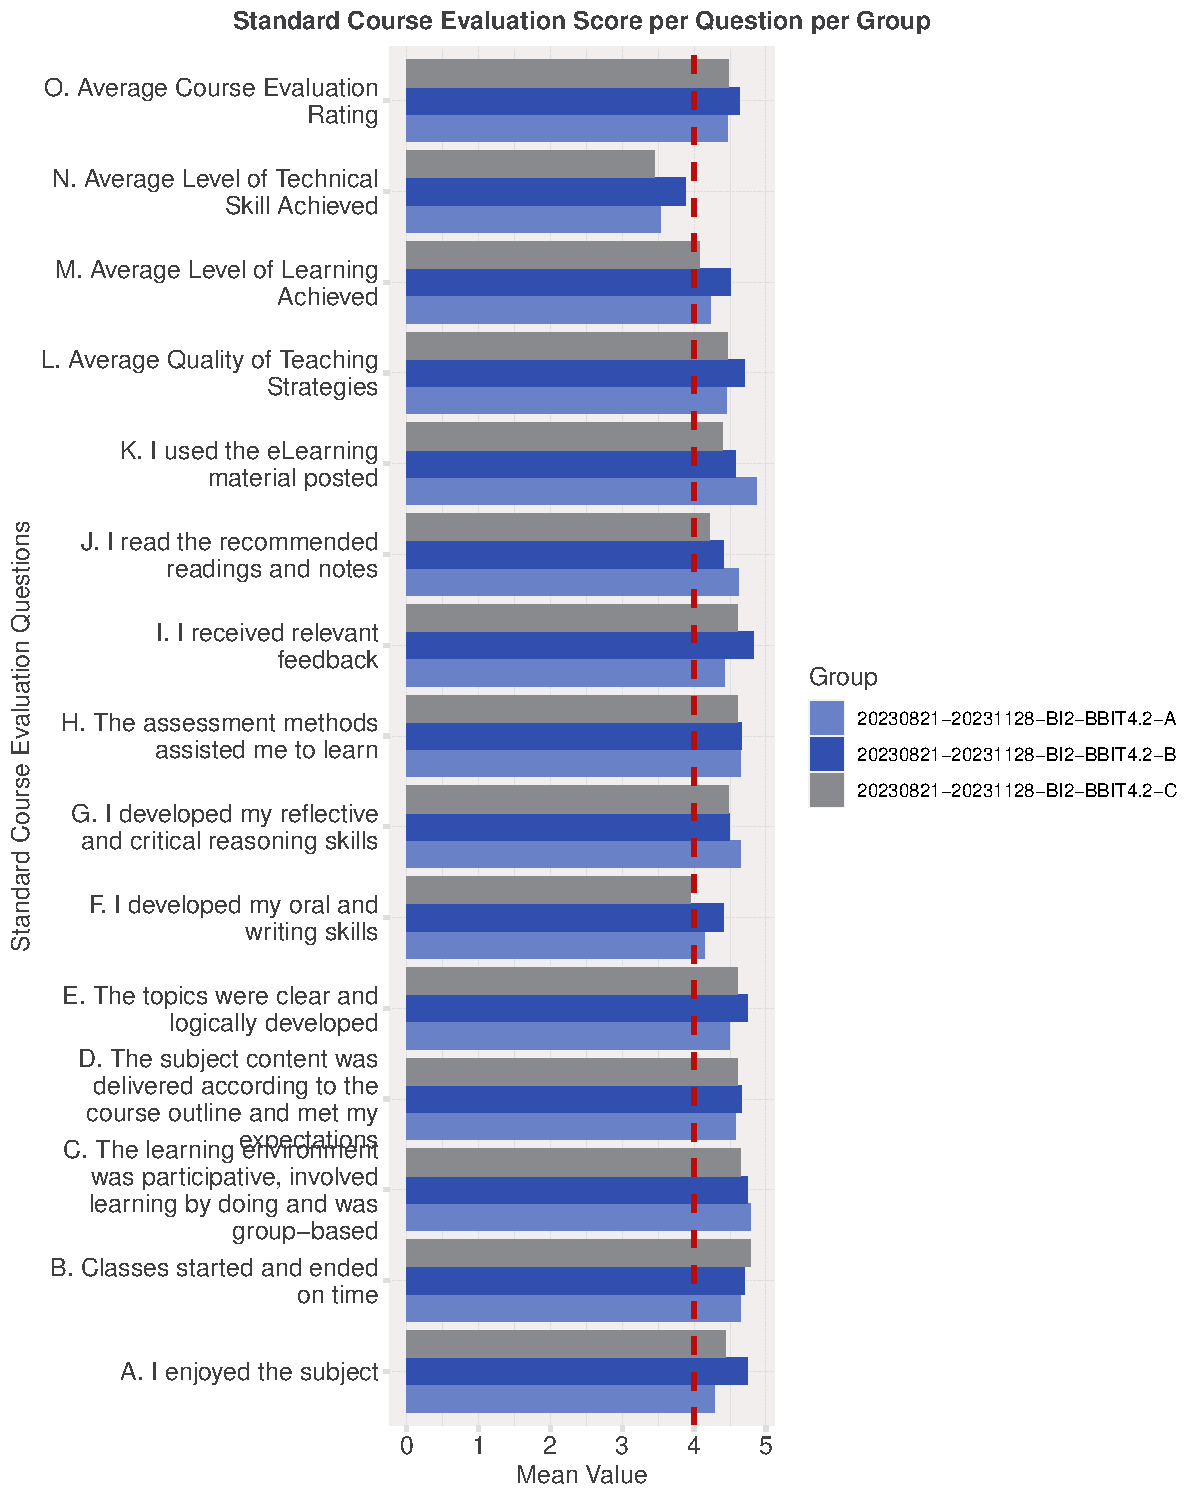
\includegraphics{10.b.BBT4206-End-SemesterCourseEvaluation-20230821-20231128-BI2-BBIT4-2_files/figure-latex/VisualizationsForCourseEvaluationResultsperClassGroup-1.pdf}

\newpage

The \textbf{``Average Course Evaluation Rating''} variable in the plot
below indicates the score \textbf{per gender} with a baseline of 4/5.

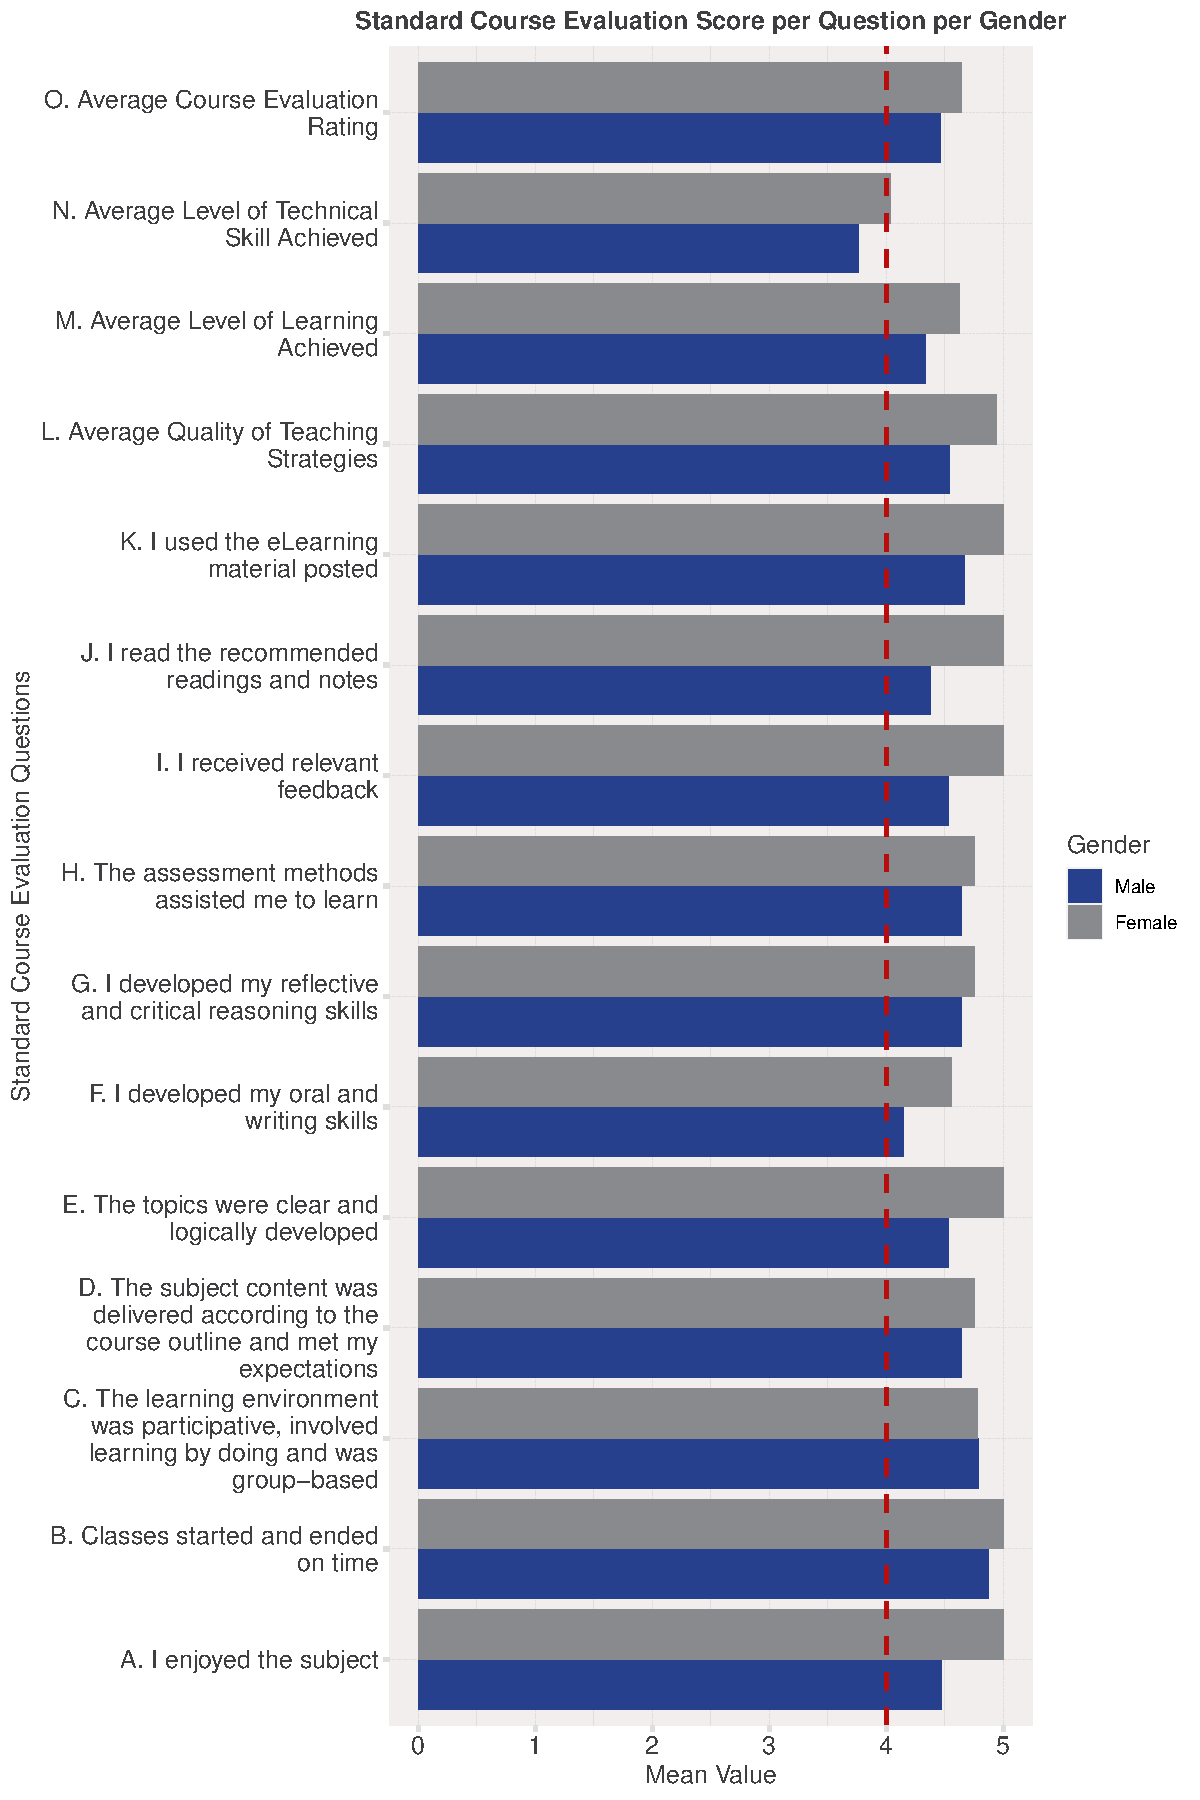
\includegraphics{10.b.BBT4206-End-SemesterCourseEvaluation-20230821-20231128-BI2-BBIT4-2_files/figure-latex/VisualizationsForCourseEvaluationResultsperGender-1.pdf}

\newpage

The plot below presents a drill-down of the class group into
\textbf{regular and exempt} students:

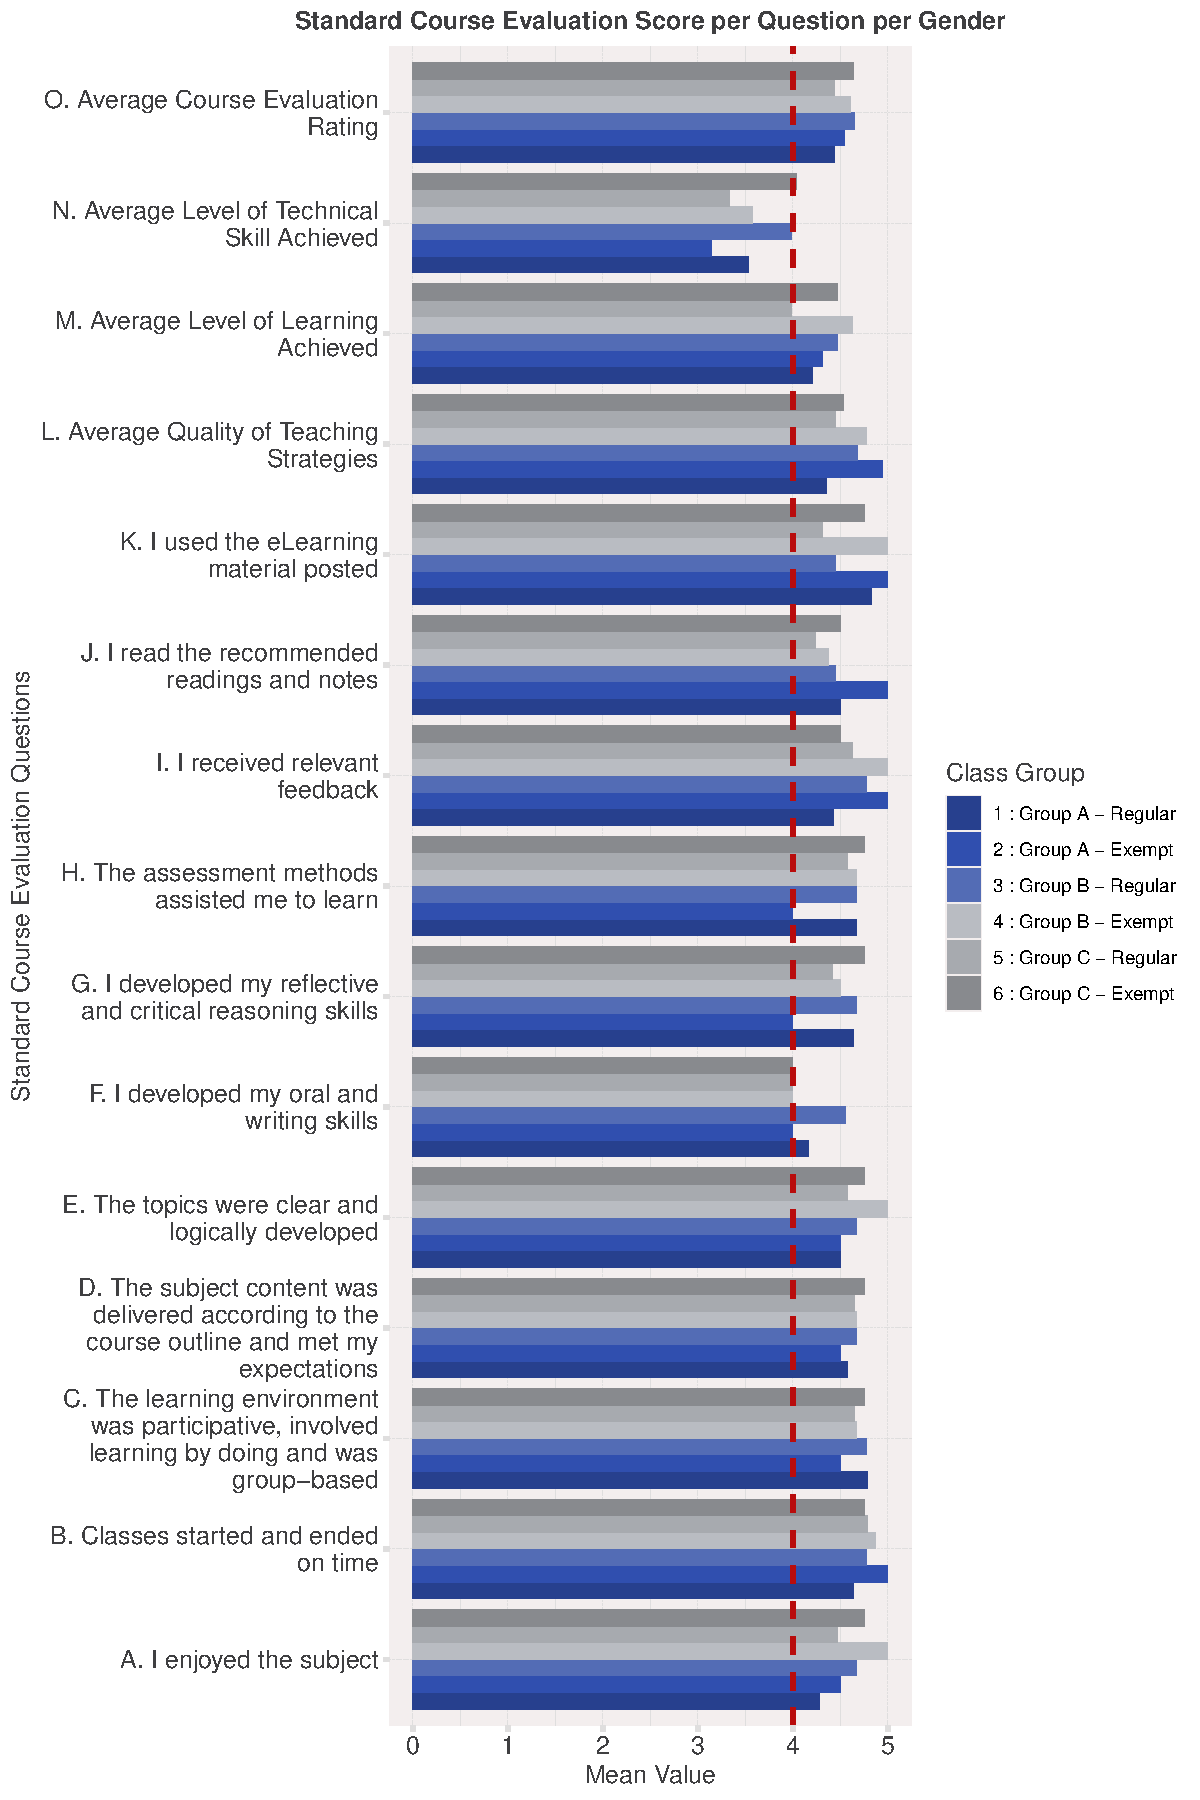
\includegraphics{10.b.BBT4206-End-SemesterCourseEvaluation-20230821-20231128-BI2-BBIT4-2_files/figure-latex/VisualizationsForCourseEvaluationResultsperGroup-1.pdf}

\newpage

Note that the 22 indicated as ``NA'' are all in Group A. Group A
students filled in the course evaluation form before the question was
set. Out of those asked, 98\% do not regret the choice to take the
Business Intelligence Option instead of the Computer Networking Option
in their final year.

\begin{verbatim}
## # A tibble: 3 x 2
##   `Do you regret choosing the BI Option?` Number
##   <chr>                                    <int>
## 1 1 : Yes                                      2
## 2 2 : No                                      83
## 3 <NA>                                        22
\end{verbatim}

\newpage

\subsection{Correlations}\label{correlations}

The specific correlation values are presented below:

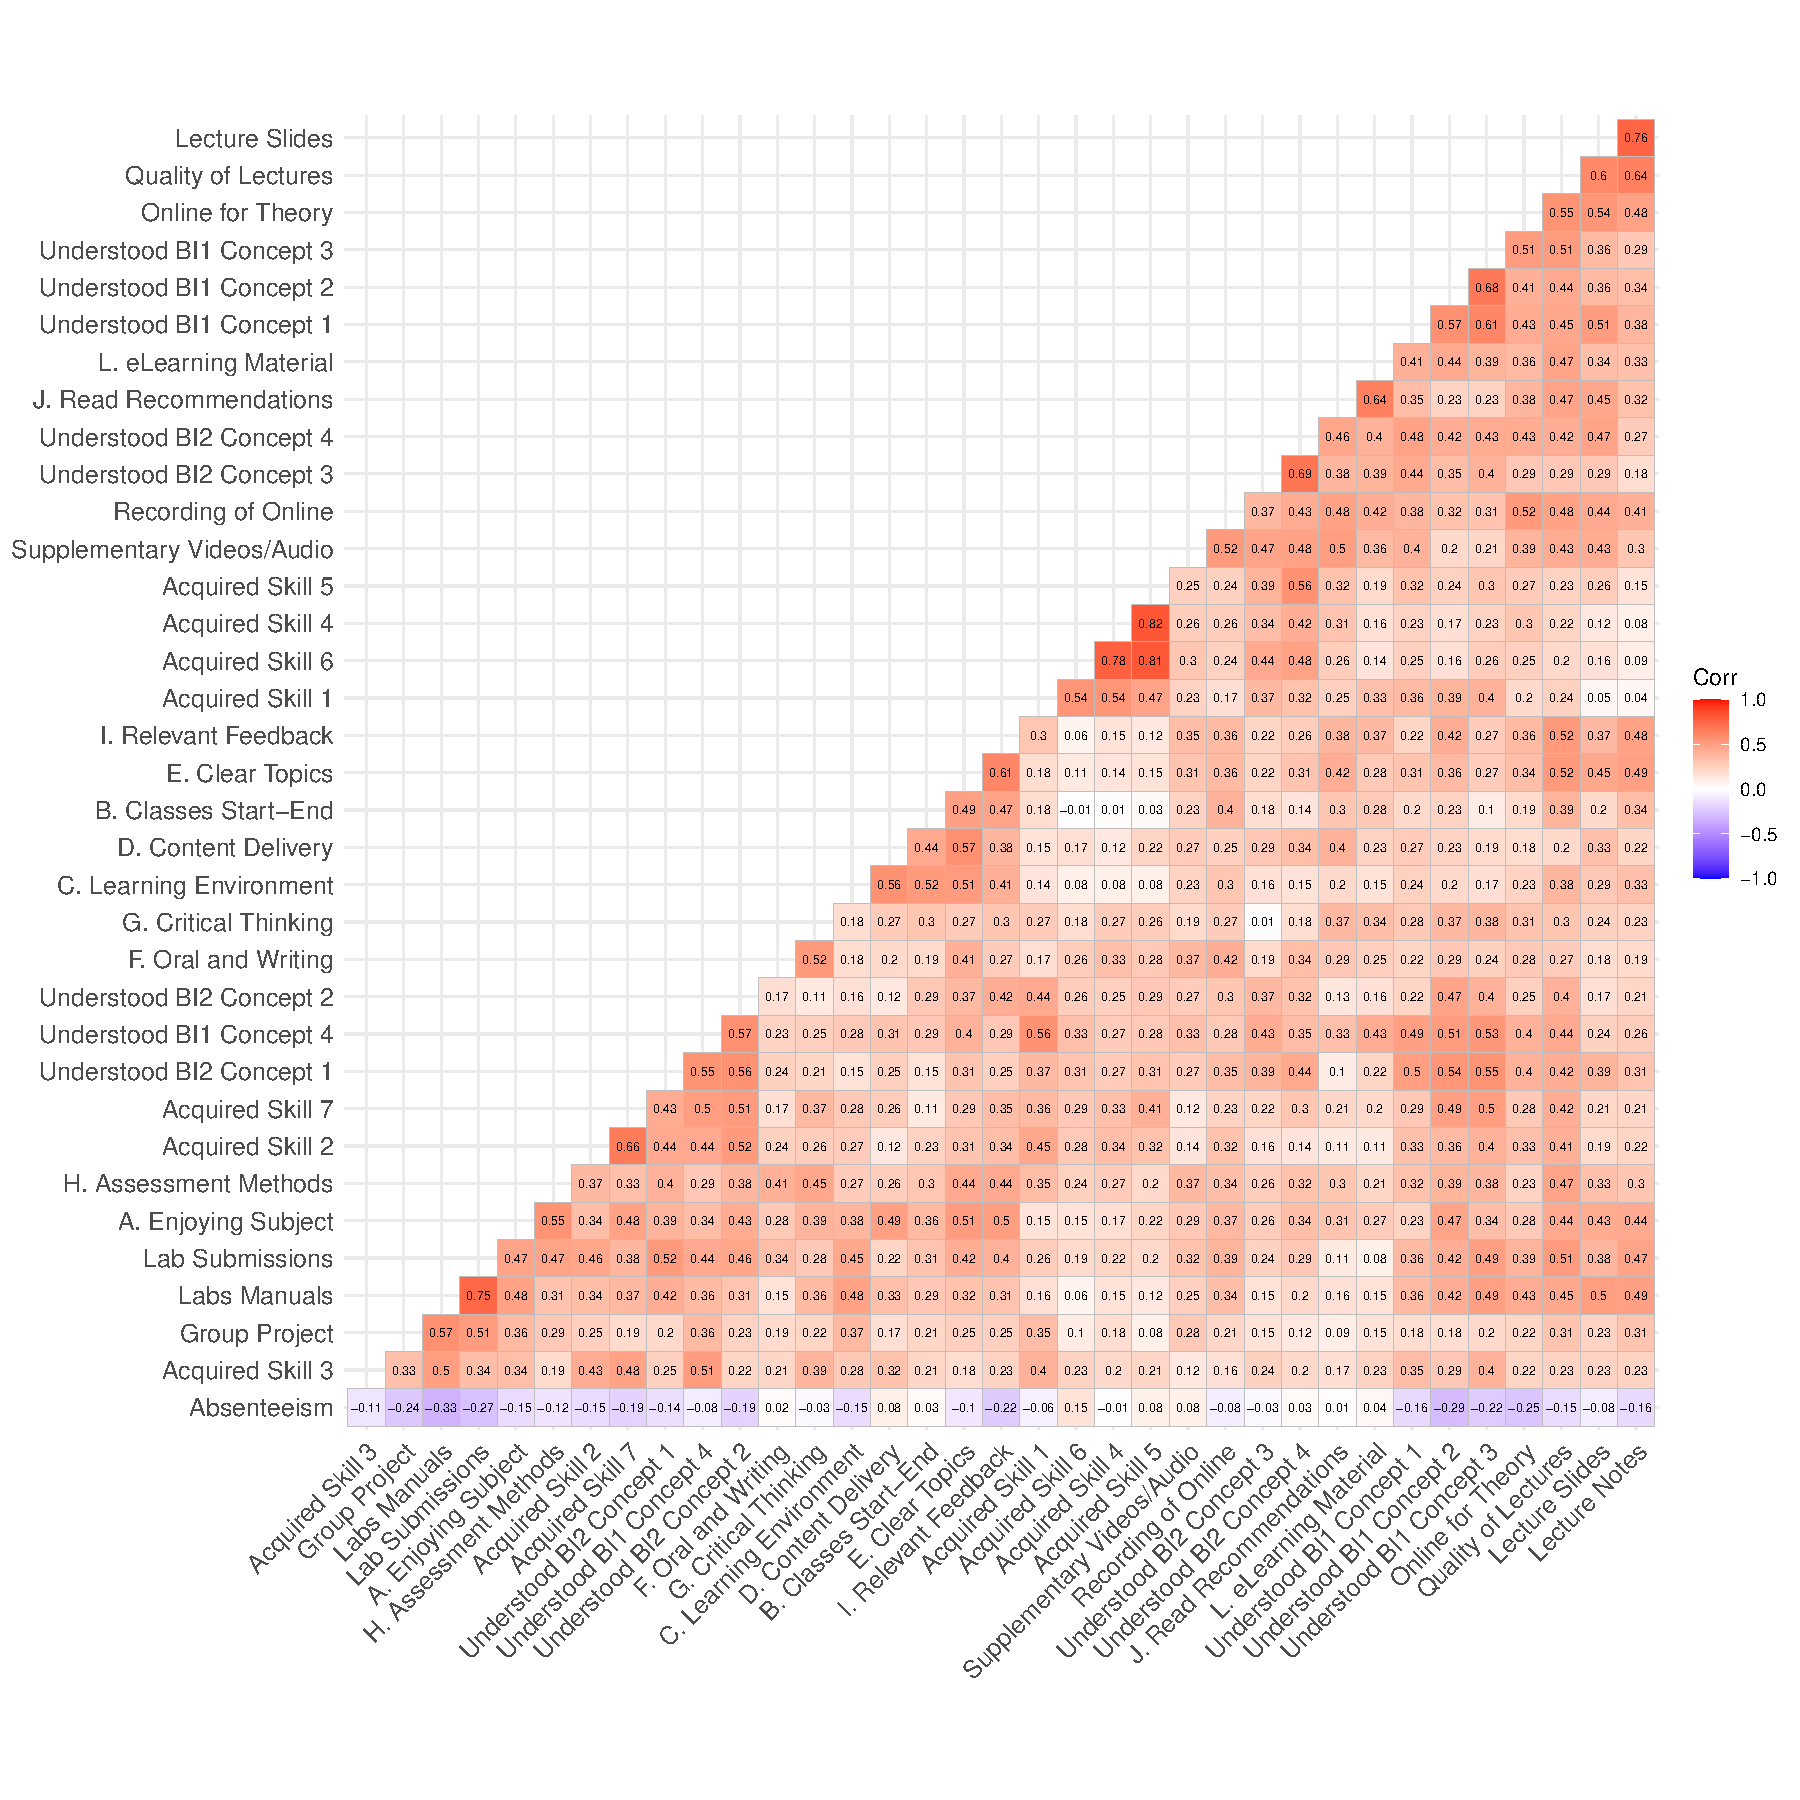
\includegraphics{10.b.BBT4206-End-SemesterCourseEvaluation-20230821-20231128-BI2-BBIT4-2_files/figure-latex/CorrelationMatrixWithFigures-1.pdf}

\subsubsection{Interesting Correlations}\label{interesting-correlations}

The following are hypothetical statements given that ``correlation does
not imply causation''.

\begin{itemize}
\item
  \textbf{.81 correlation} between ``Acquired Skill 6 (ClickHouse)'' and
  ``Acquired Skill 5 (ksqlDB)'': \emph{The two technologies are related
  and taught in the same lab (Data Engineering).}
\item
  \textbf{.82 correlation} between ``Acquired Skill 4 (Kafka)'' and
  ``Acquired Skill 5 (ksqlDB)'': \emph{The two technologies are related
  and taught in the same lab and concept (Data Engineering).}
\item
  \textbf{.78 correlation} between ``Acquired Skill 6 (ClickHouse)'' and
  ``Acquired Skill 4 (Kafka)'': \emph{The two technologies are related
  and taught in the same lab (Data Engineering).}
\item
  \textbf{.75 correlation} between ``Lab Manuals (Lab manuals that
  outline the steps to follow during the labs)'' and ``Lab Submissions
  (Required lab work submissions at the end of each lab manual that
  outline the activity to be done on your own)'': \emph{The more the
  effort to clearly outline the steps to be done in a lab manual, the
  more impact it has on the students' learning.}
\item
  \textbf{.76 correlation} between ``The quality of lecture slides'' and
  ``the quality of lecture notes on some of the slides: \emph{The higher
  the quality of the slides, the higher the quality of the notes on some
  of the slides.}
\end{itemize}

\begin{enumerate}
\def\labelenumi{(\arabic{enumi})}
\tightlist
\item
  A \textbf{.76 correlation} between ``The quality of lecture slides''
  and ``the quality of lecture notes on some of the slides.
\end{enumerate}

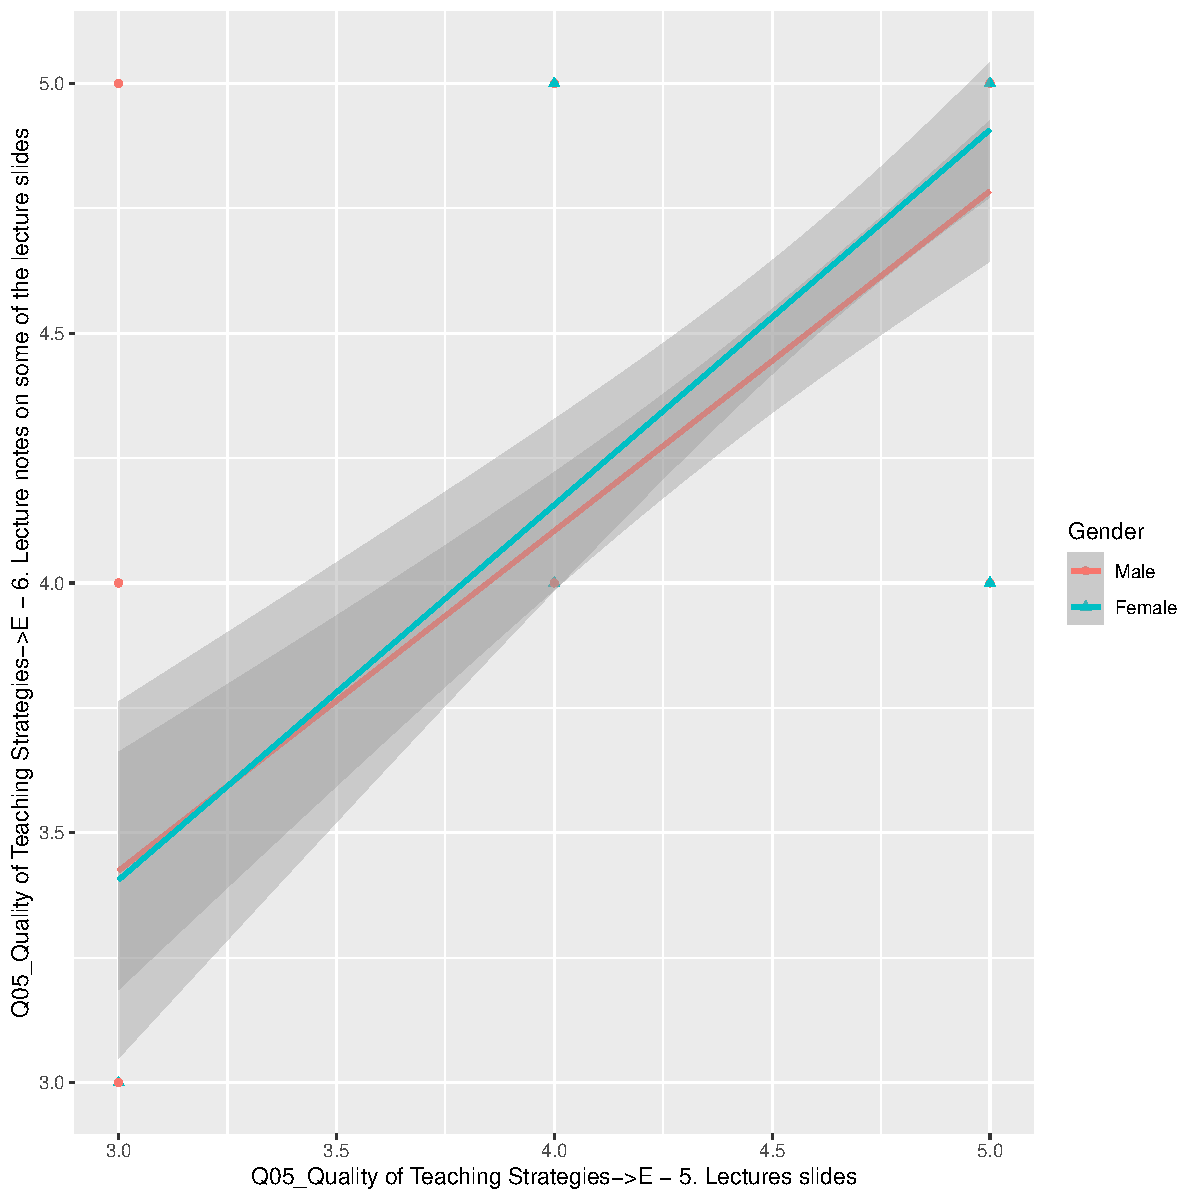
\includegraphics{10.b.BBT4206-End-SemesterCourseEvaluation-20230821-20231128-BI2-BBIT4-2_files/figure-latex/DrillDownCorr1-1.pdf}

\newpage

\begin{enumerate}
\def\labelenumi{(\arabic{enumi})}
\setcounter{enumi}{1}
\tightlist
\item
  A \textbf{.75 correlation} between ``Lab Manuals (Lab manuals that
  outline the steps to follow during the labs)'' and ``Lab Submissions
  (Required lab work submissions at the end of each lab manual that
  outline the activity to be done on your own)''.
\end{enumerate}

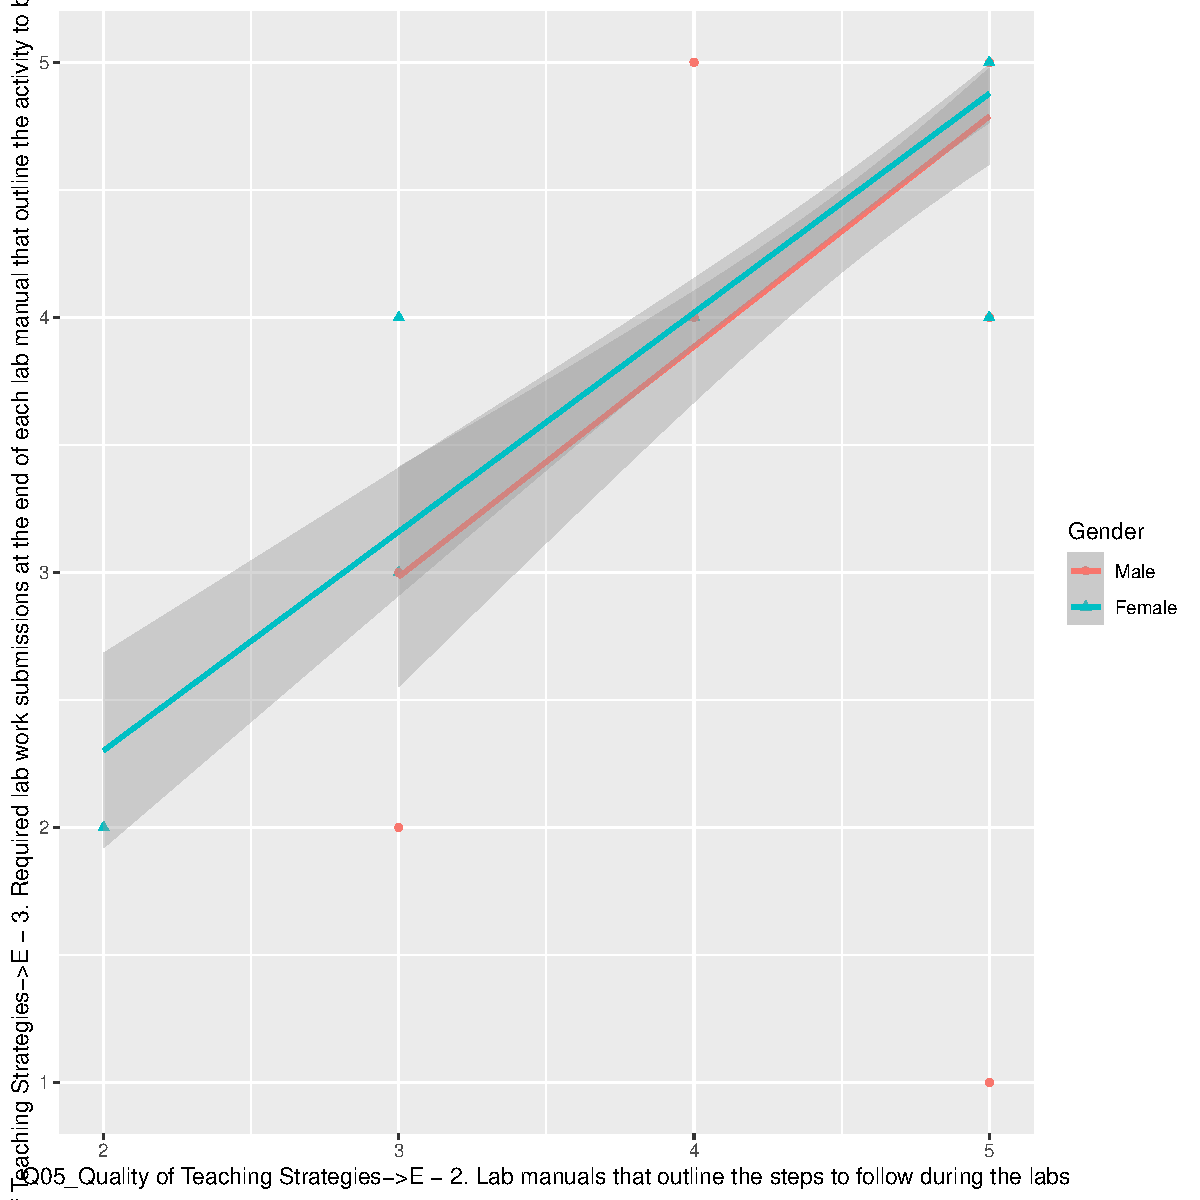
\includegraphics{10.b.BBT4206-End-SemesterCourseEvaluation-20230821-20231128-BI2-BBIT4-2_files/figure-latex/DrillDownCorr2-1.pdf}

\newpage

\subsubsection{Absenteeism Percentage}\label{absenteeism-percentage}

The lower the absenteeism, the more a student makes use of the lab
manuals for practical classes. And the more a student makes use of the
lab manuals, the more the lab submissions have an impact on their
overall acquisition of skills.

With this in mind, a further investigation of the \textbf{absenteeism
percentage} is presented below.

\paragraph{Absenteeism by General Class
Group}\label{absenteeism-by-general-class-group}

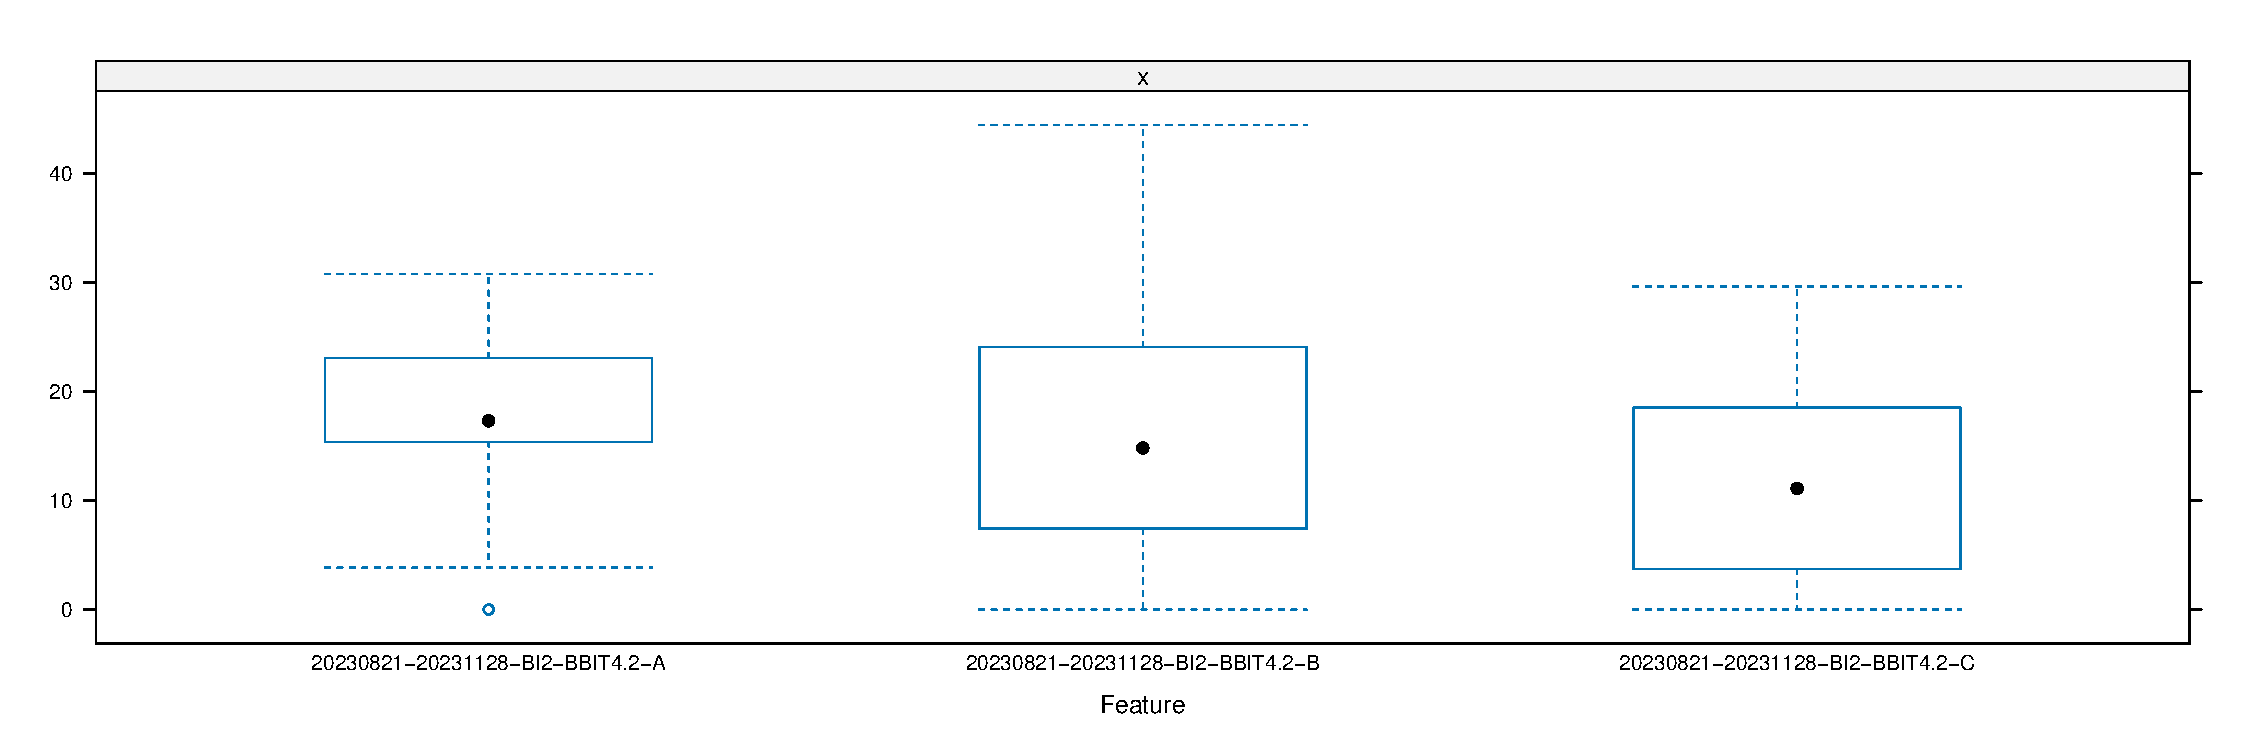
\includegraphics{10.b.BBT4206-End-SemesterCourseEvaluation-20230821-20231128-BI2-BBIT4-2_files/figure-latex/AbsenteeismBoxandWhiskerGroup-1.pdf}

\paragraph{Absenteeism by Specific Class
Group}\label{absenteeism-by-specific-class-group}

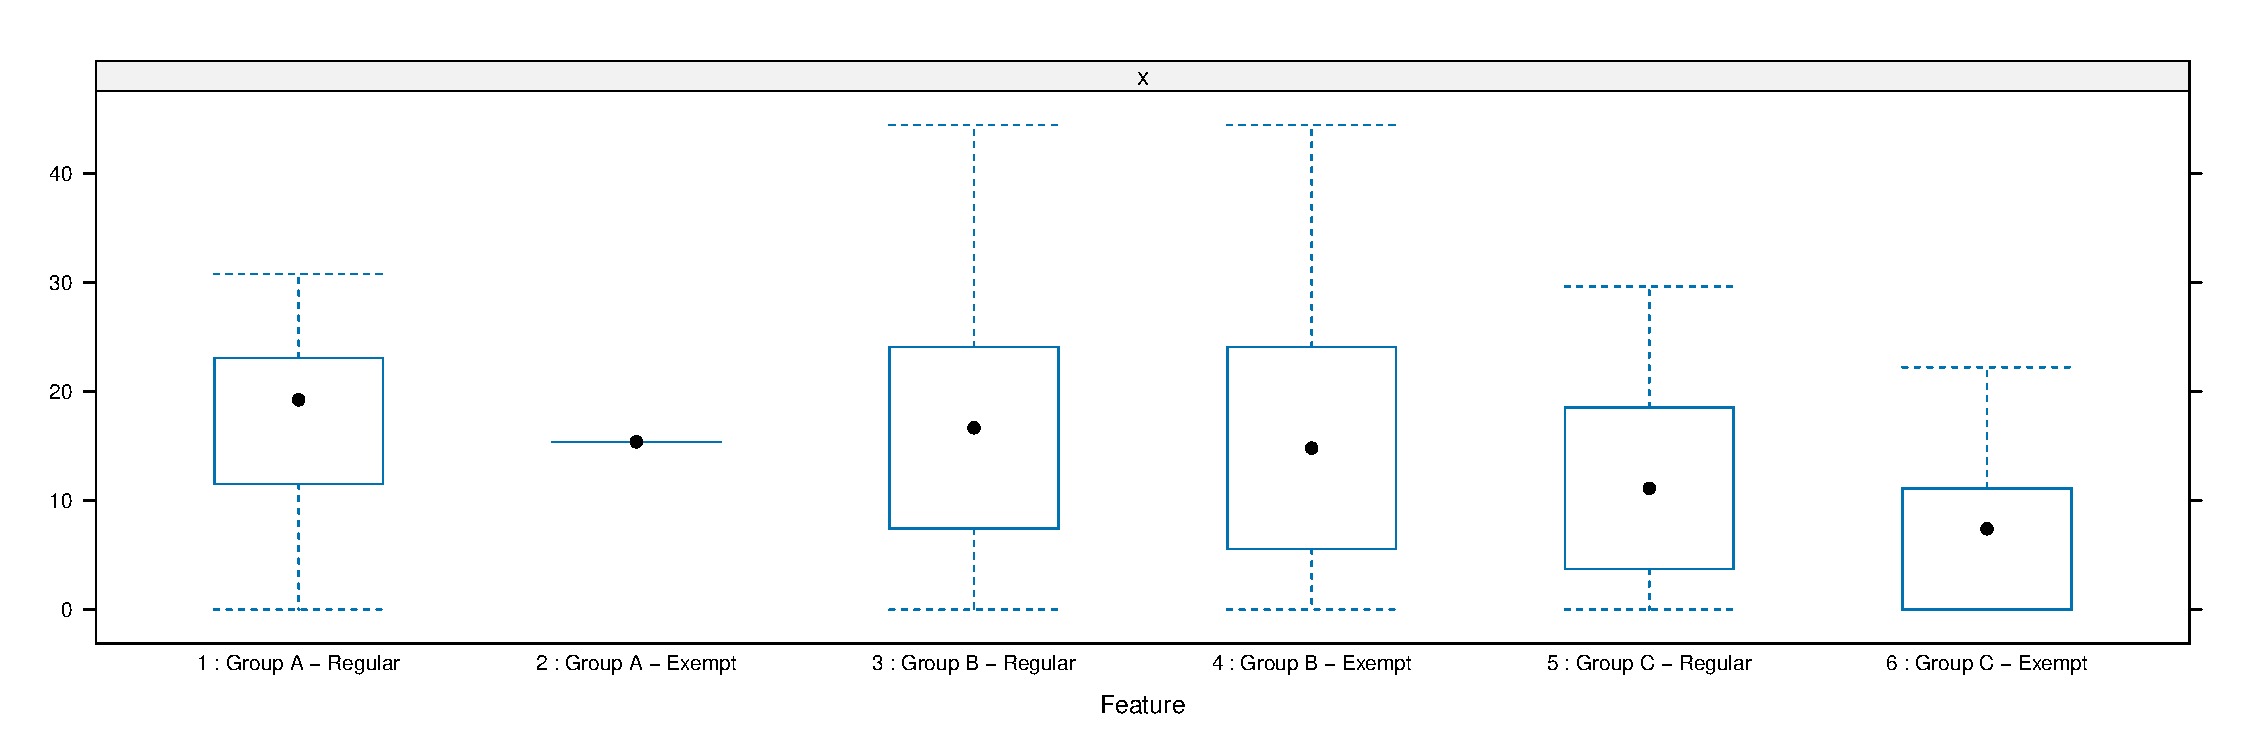
\includegraphics{10.b.BBT4206-End-SemesterCourseEvaluation-20230821-20231128-BI2-BBIT4-2_files/figure-latex/AbsenteeismBoxandWhiskerSpecificGroup-1.pdf}

\paragraph{Absenteeism by Gender}\label{absenteeism-by-gender}

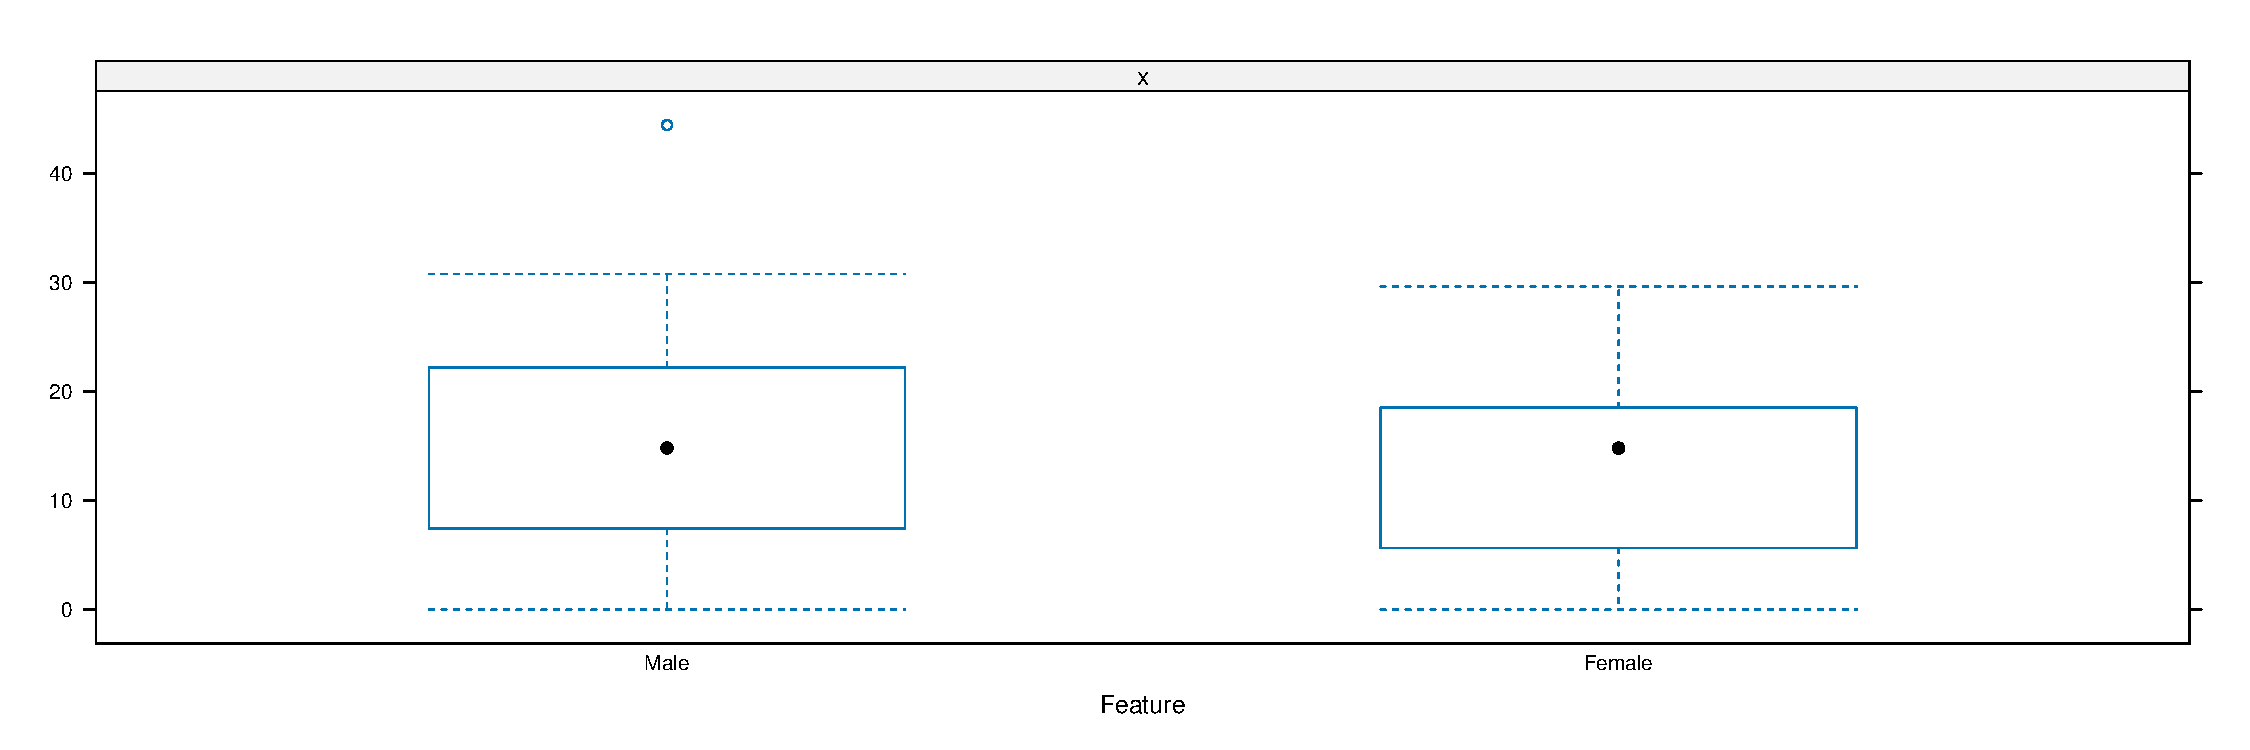
\includegraphics{10.b.BBT4206-End-SemesterCourseEvaluation-20230821-20231128-BI2-BBIT4-2_files/figure-latex/AbsenteeismBoxandWhiskerGender-1.pdf}

\newpage

\section{Qualitative Data Analysis}\label{qualitative-data-analysis}

\subsection{Sentiment Analysis
(Lexicon-Based)}\label{sentiment-analysis-lexicon-based}

The ``likes'' refer to the answer to the question, ``Write two things
you liked about the teaching and learning in this course.'' The
sentiments expressed through the ``likes'' are:

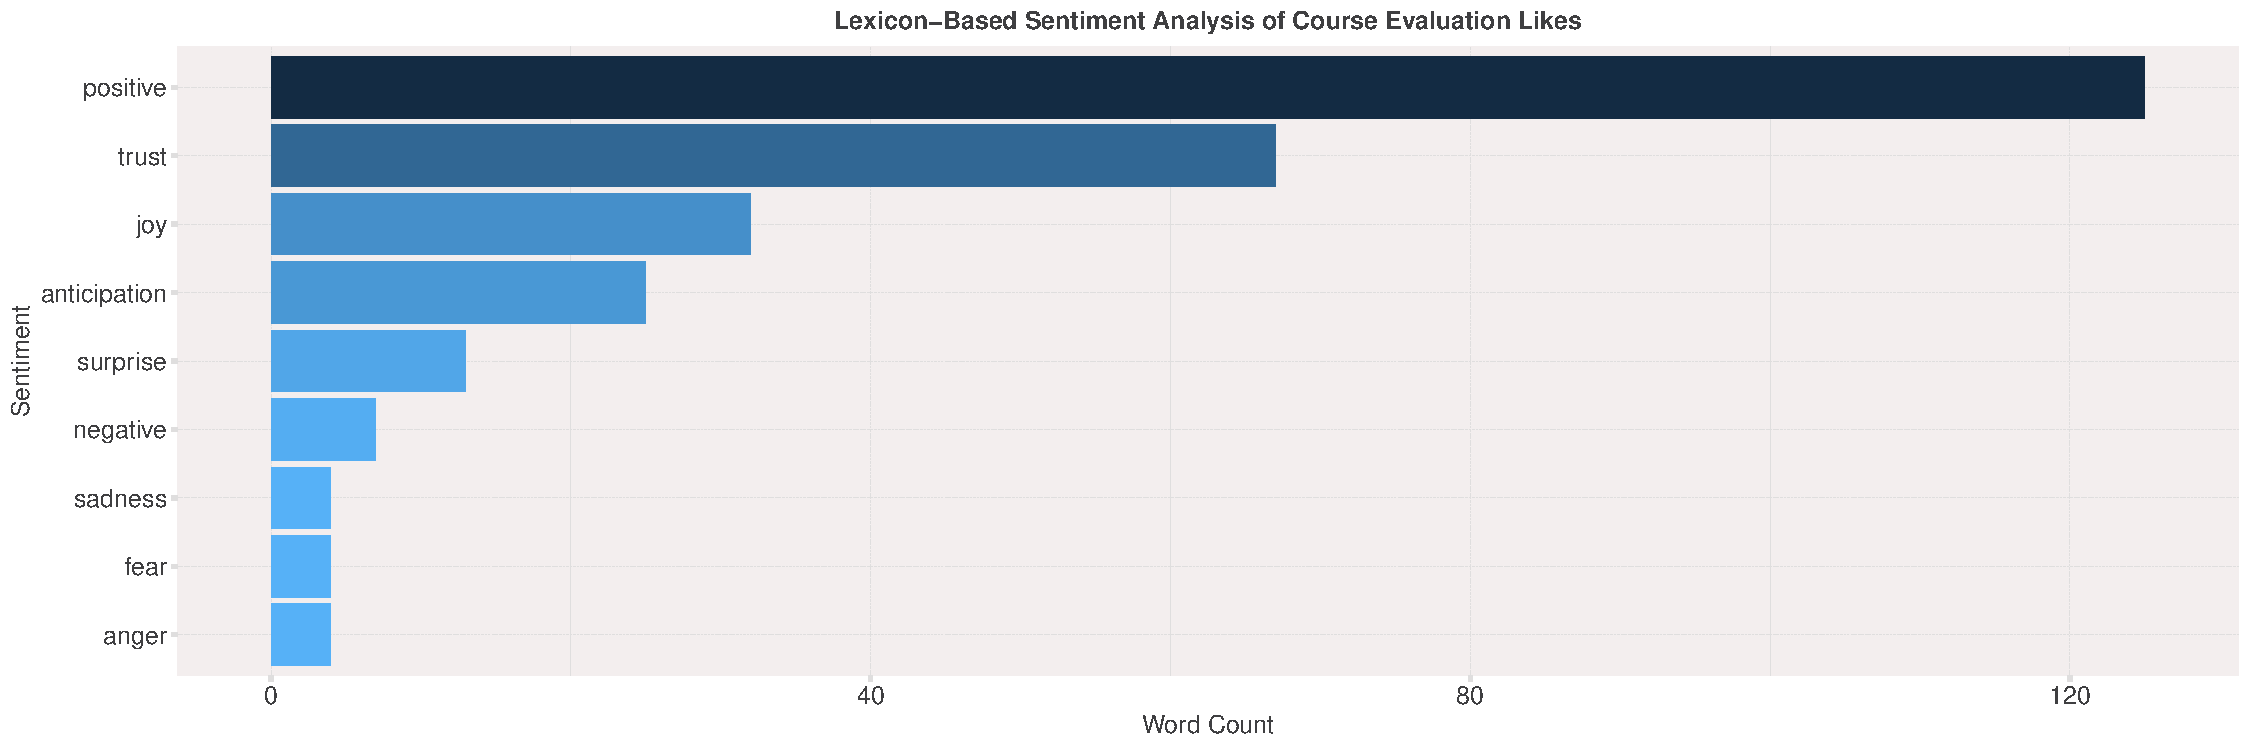
\includegraphics{10.b.BBT4206-End-SemesterCourseEvaluation-20230821-20231128-BI2-BBIT4-2_files/figure-latex/OverallSentimentForLikes-1.pdf}

The ``wishes'' refer to the answer to the question, ``Write at least one
recommendation to improve the teaching and learning in this course (for
future classes)''. The sentiments expressed through the ``wishes'' are:

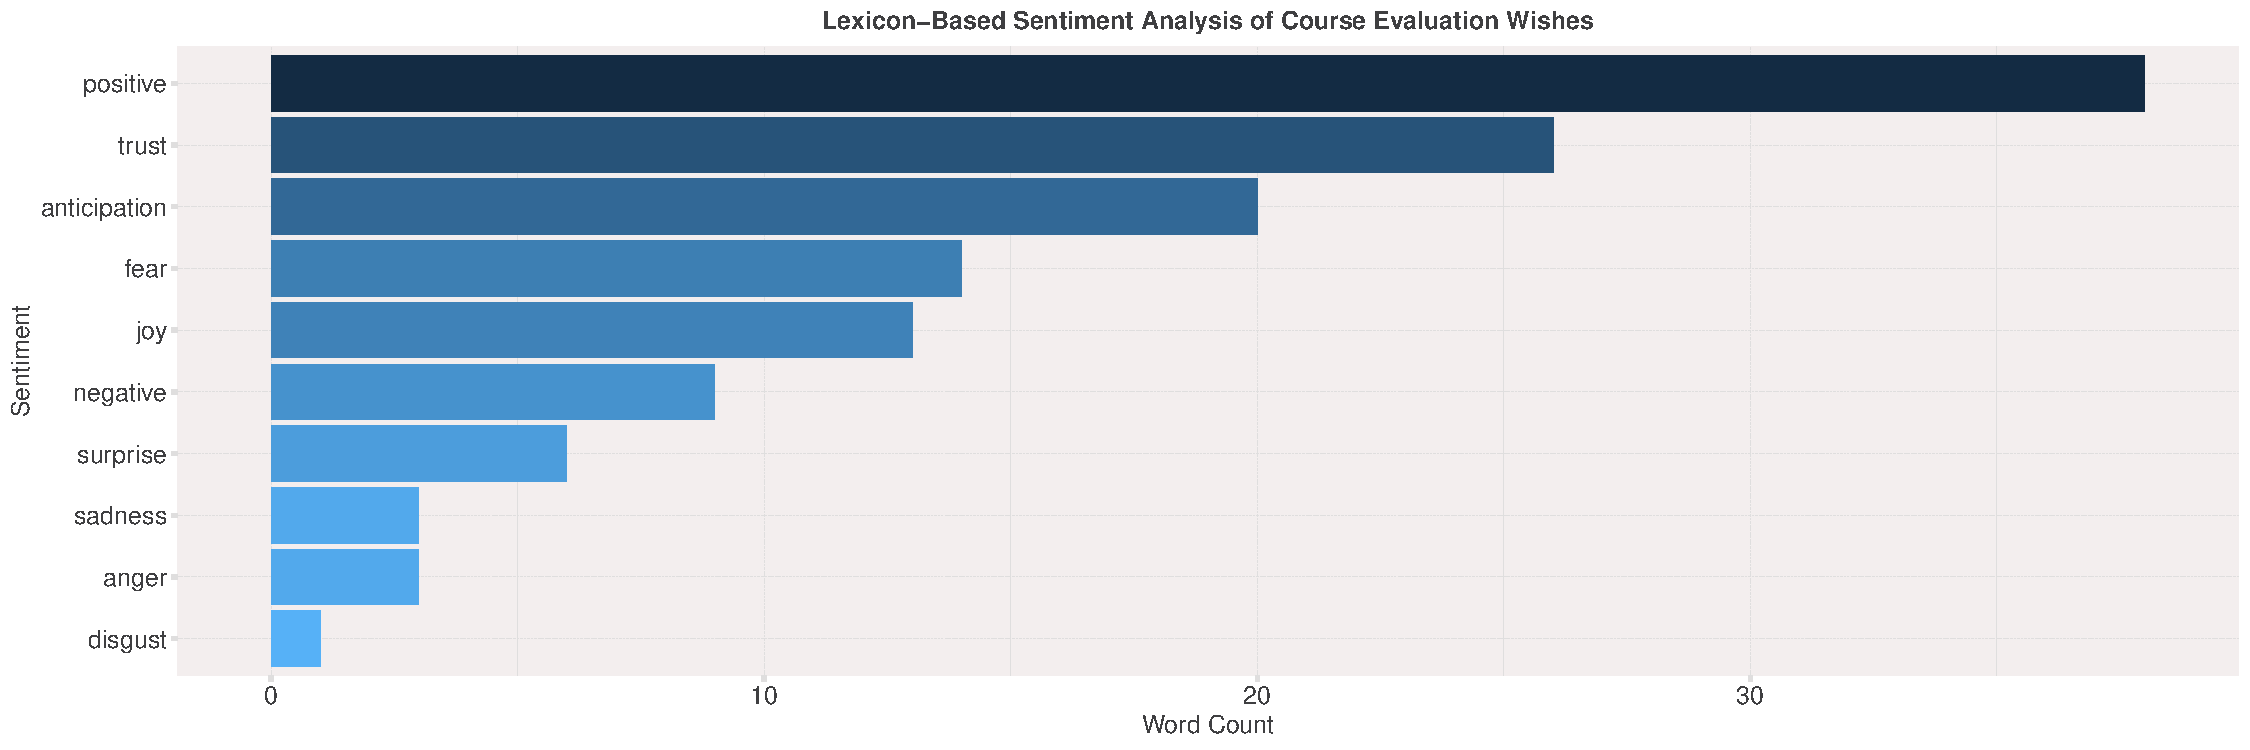
\includegraphics{10.b.BBT4206-End-SemesterCourseEvaluation-20230821-20231128-BI2-BBIT4-2_files/figure-latex/OverallSentimentForWishes-1.pdf}

\newpage

Chord Diagram of Likes per Class Group:

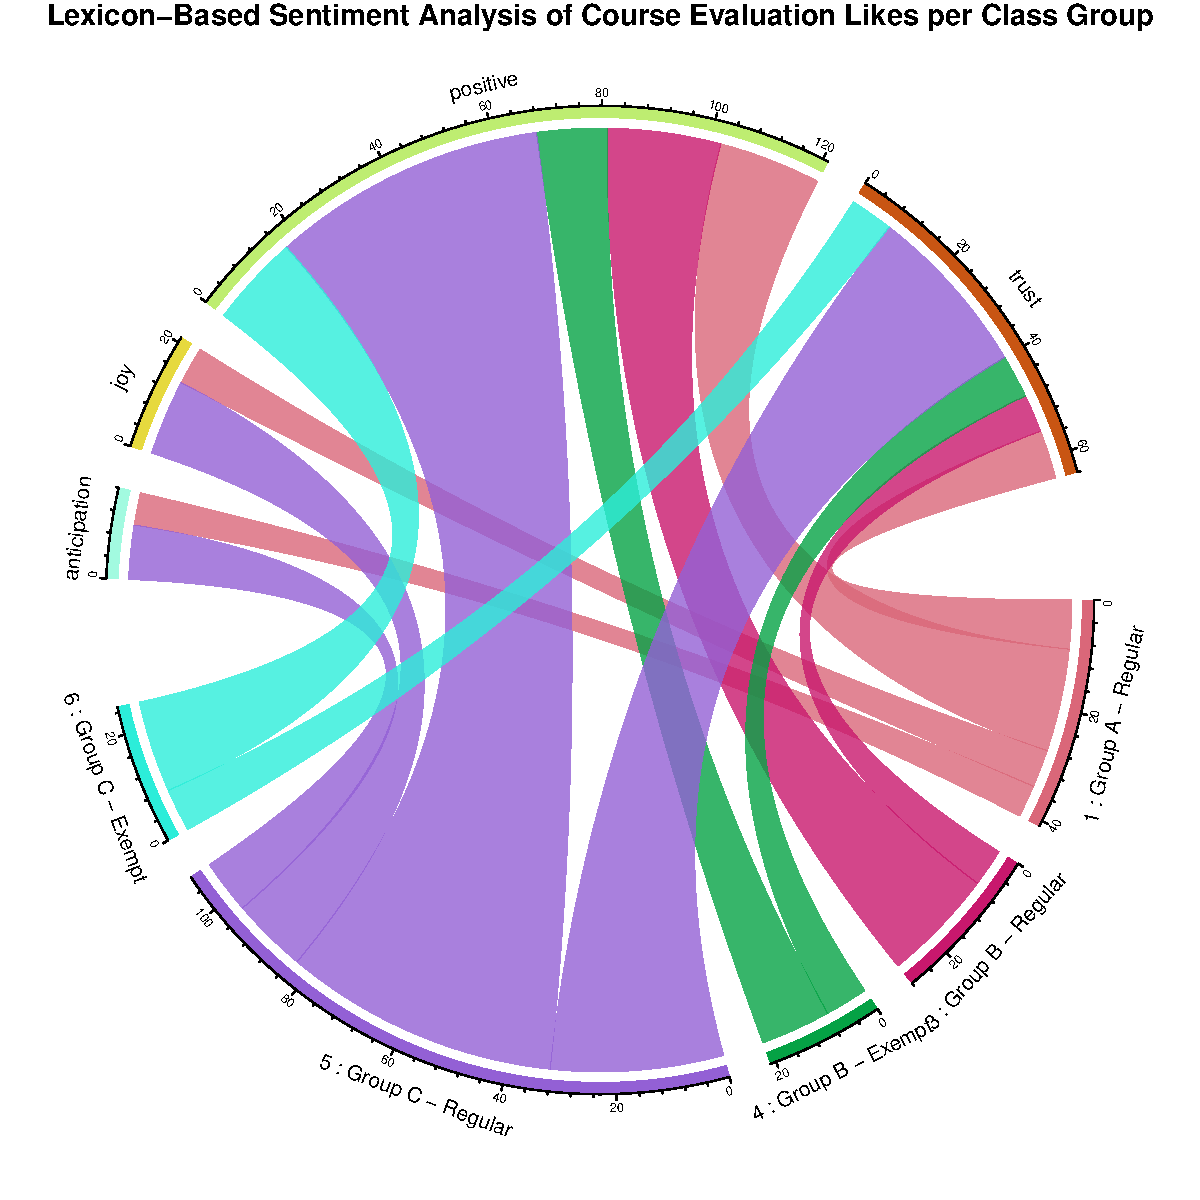
\includegraphics{10.b.BBT4206-End-SemesterCourseEvaluation-20230821-20231128-BI2-BBIT4-2_files/figure-latex/ChordDiagramLikesPerGroup-1.pdf}

\newpage

Chord Diagram of Likes per Class Gender:

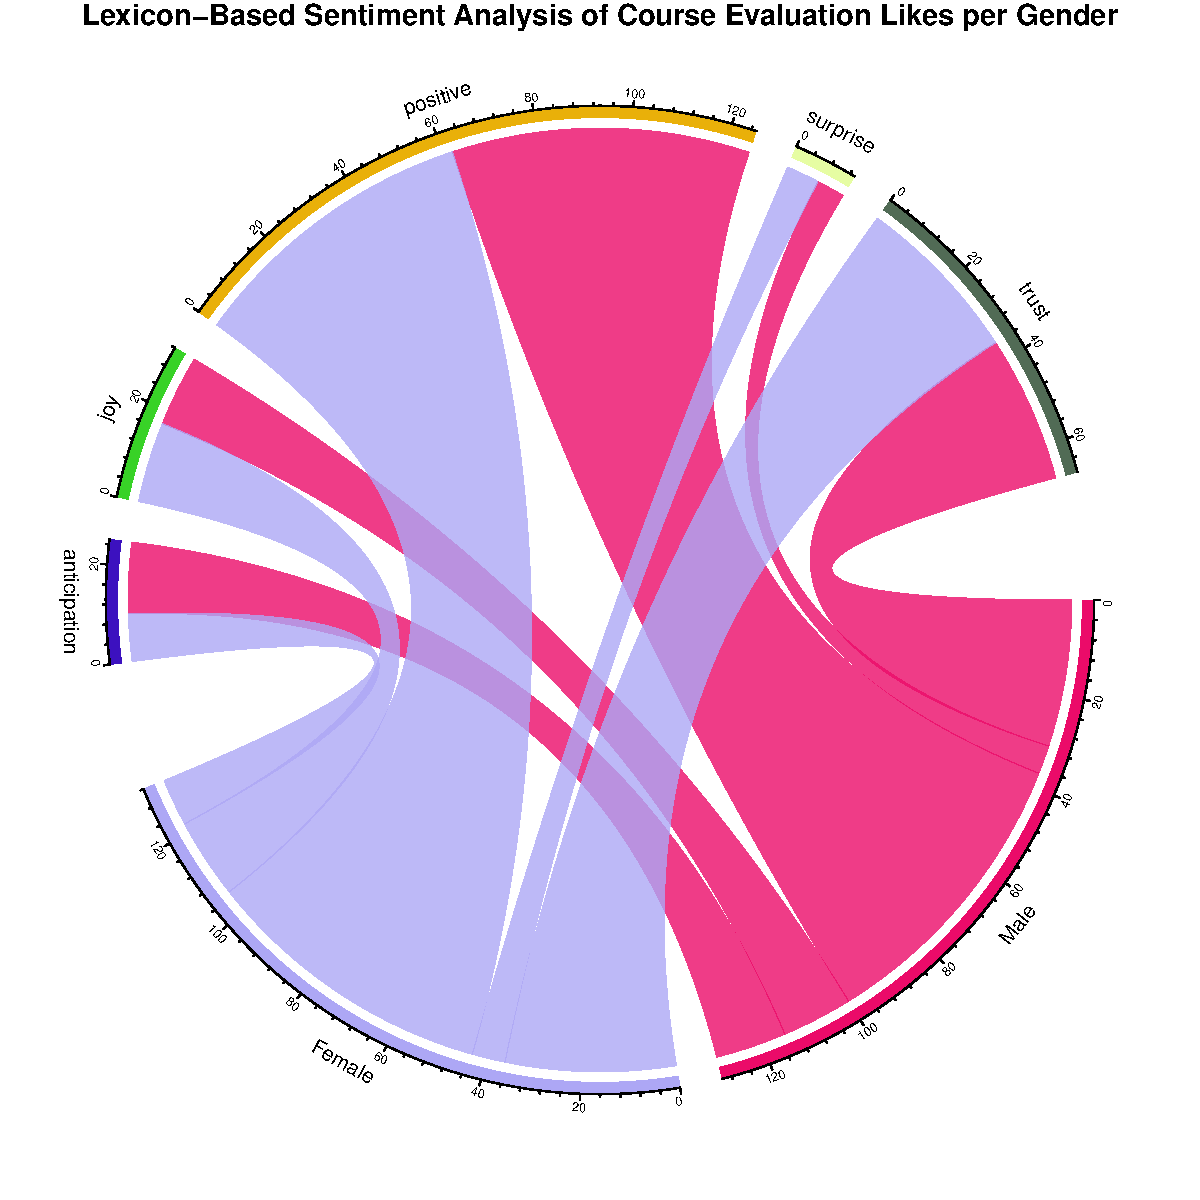
\includegraphics{10.b.BBT4206-End-SemesterCourseEvaluation-20230821-20231128-BI2-BBIT4-2_files/figure-latex/ChordDiagramLikesPerGender-1.pdf}

\newpage

Chord Diagram of Wishes per Class Group:

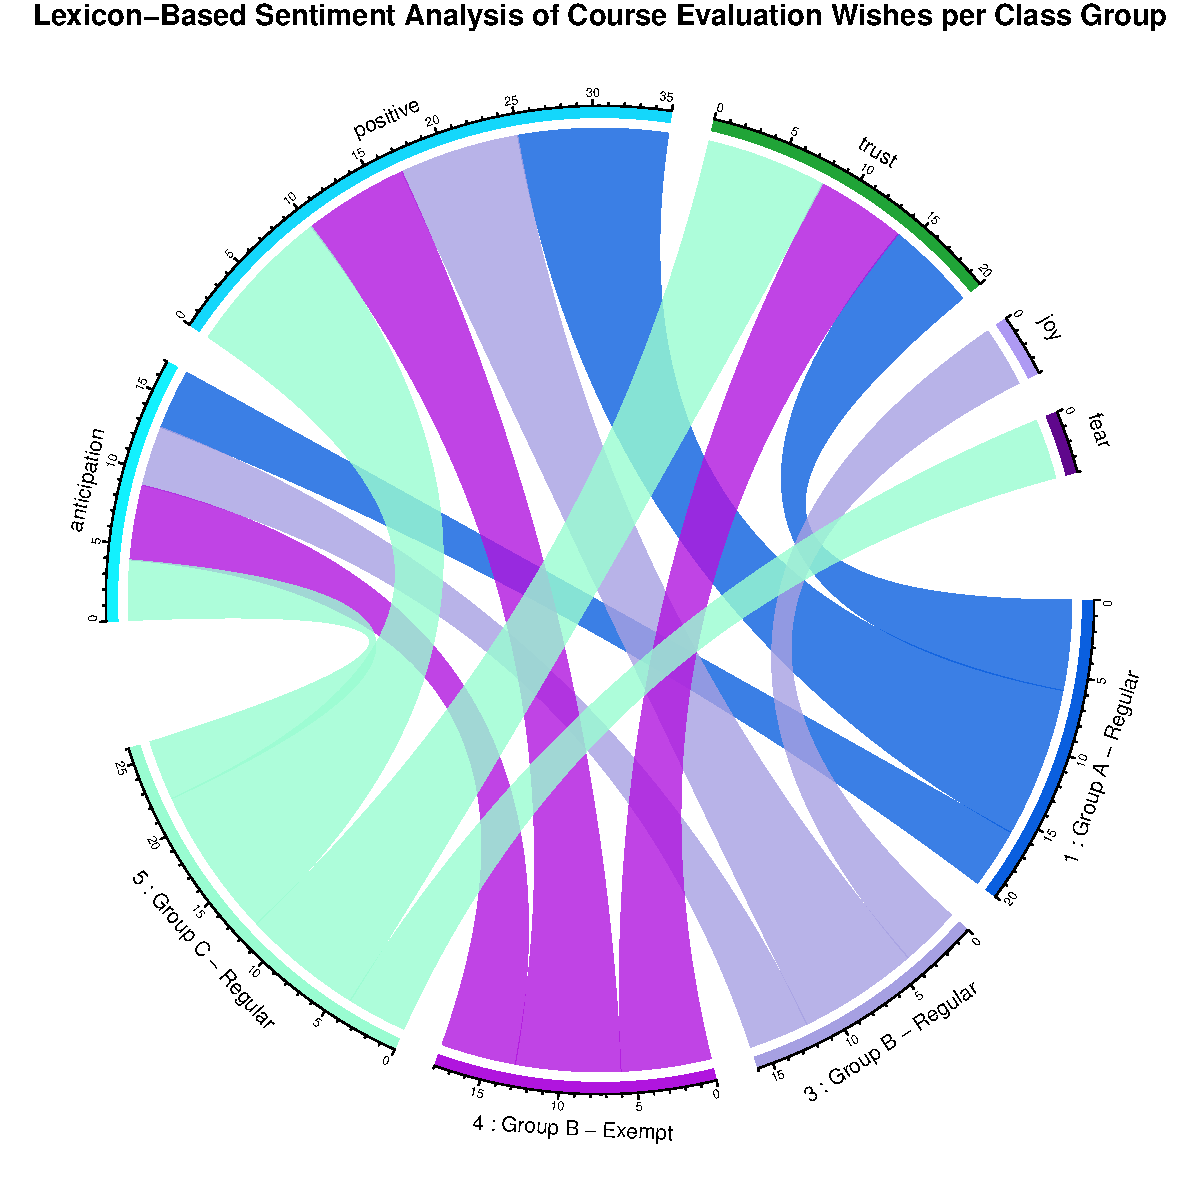
\includegraphics{10.b.BBT4206-End-SemesterCourseEvaluation-20230821-20231128-BI2-BBIT4-2_files/figure-latex/ChordDiagramPerGroup_Wishes-1.pdf}

\newpage

Chord Diagram of Wishes per Gender:

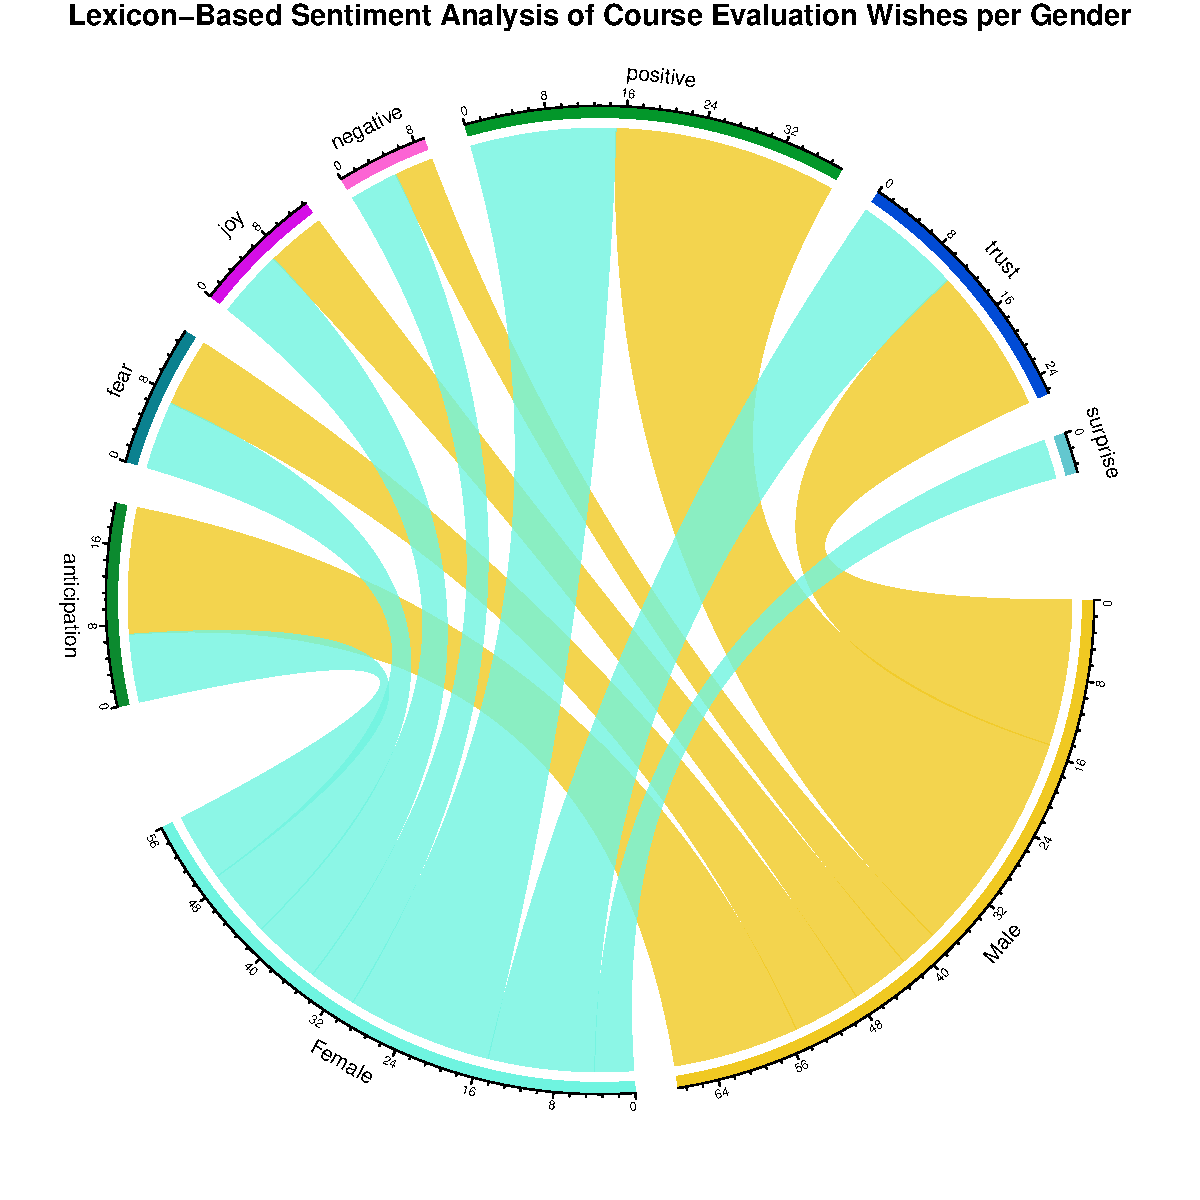
\includegraphics{10.b.BBT4206-End-SemesterCourseEvaluation-20230821-20231128-BI2-BBIT4-2_files/figure-latex/ChordDiagramPerGender_Wishes-1.pdf}

\newpage

\subsection{Topic Modelling (Latent Dirichlet Allocation (LDA)
based)}\label{topic-modelling-latent-dirichlet-allocation-lda-based}

The goal of topic modelling is to identify latent (hidden) terms
(topics) in the students' course evaluation textual feedback. In this
case, a topic is a mixture of words and a student's textual feedback is
a combination of one or more topics (mixed-membership model).

The 2 topics for the ``likes'' (as guided by the LDA model) are:

\begin{enumerate}
\def\labelenumi{\arabic{enumi}.}
\item
  Topic 1: Well-Explained Lectures
\item
  Topic 2: Collaborative Environment
\item
  Topic 3: Well-Taught for Ease of Understanding
\end{enumerate}

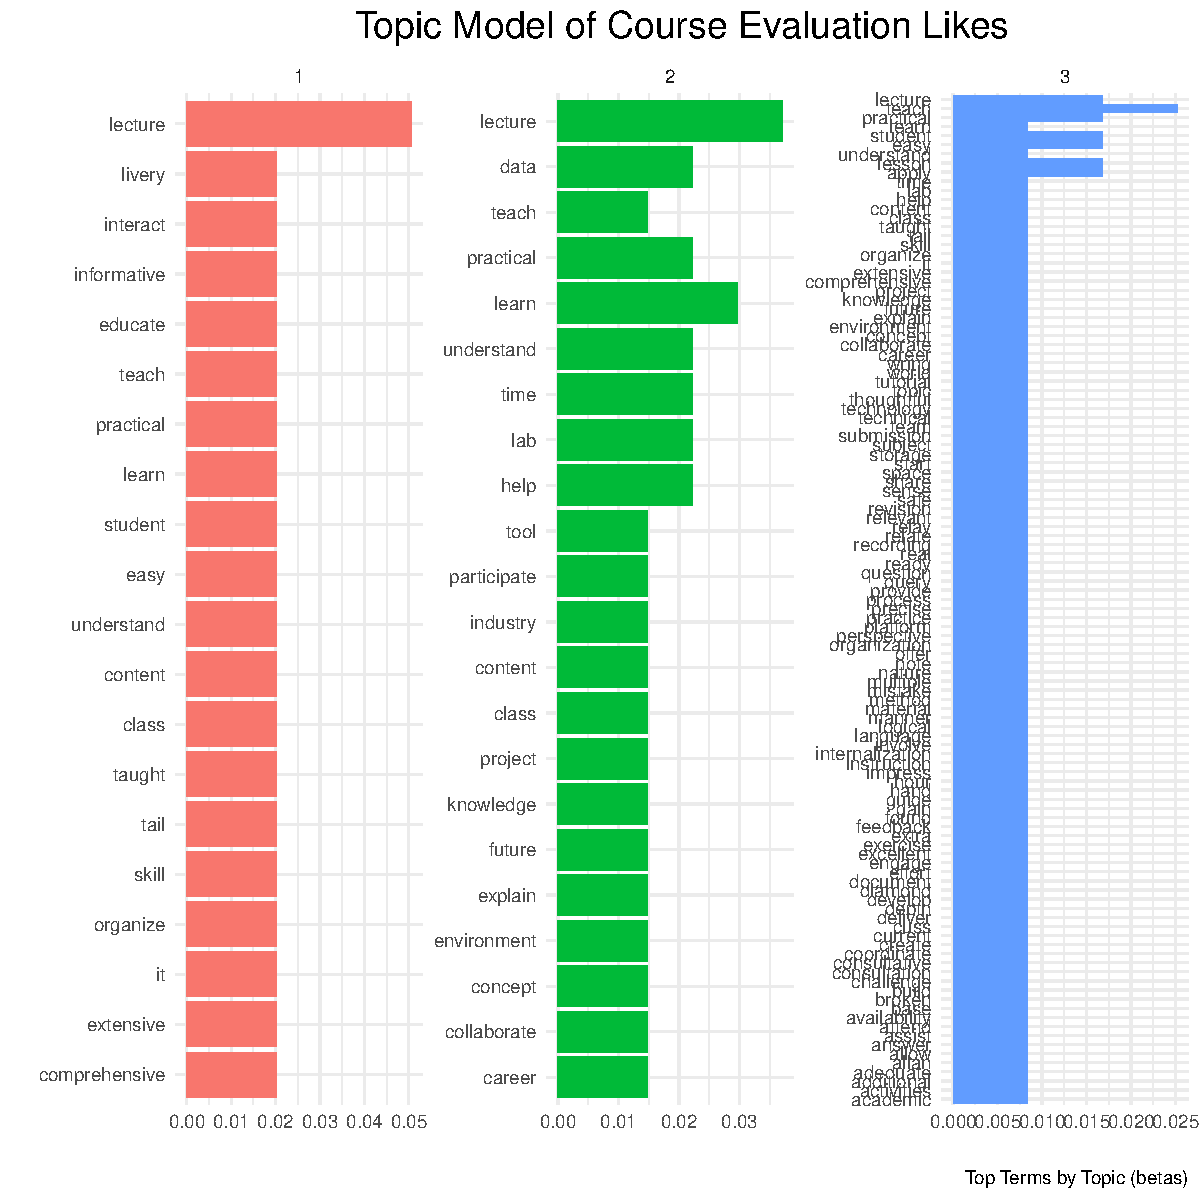
\includegraphics{10.b.BBT4206-End-SemesterCourseEvaluation-20230821-20231128-BI2-BBIT4-2_files/figure-latex/visualizations_for_likes_topic_modelling-1.pdf}

\newpage

The 5 topics for the ``wishes'' (as guided by the LDA model) are:

\begin{enumerate}
\def\labelenumi{\arabic{enumi}.}
\item
  Topic 1: Reduce the Workload
\item
  Topic 2: Reduce the Complexity of the Labs
\item
  Topic 3: Application of Data Engineering
\item
  Topic 4: Application of Python
\end{enumerate}

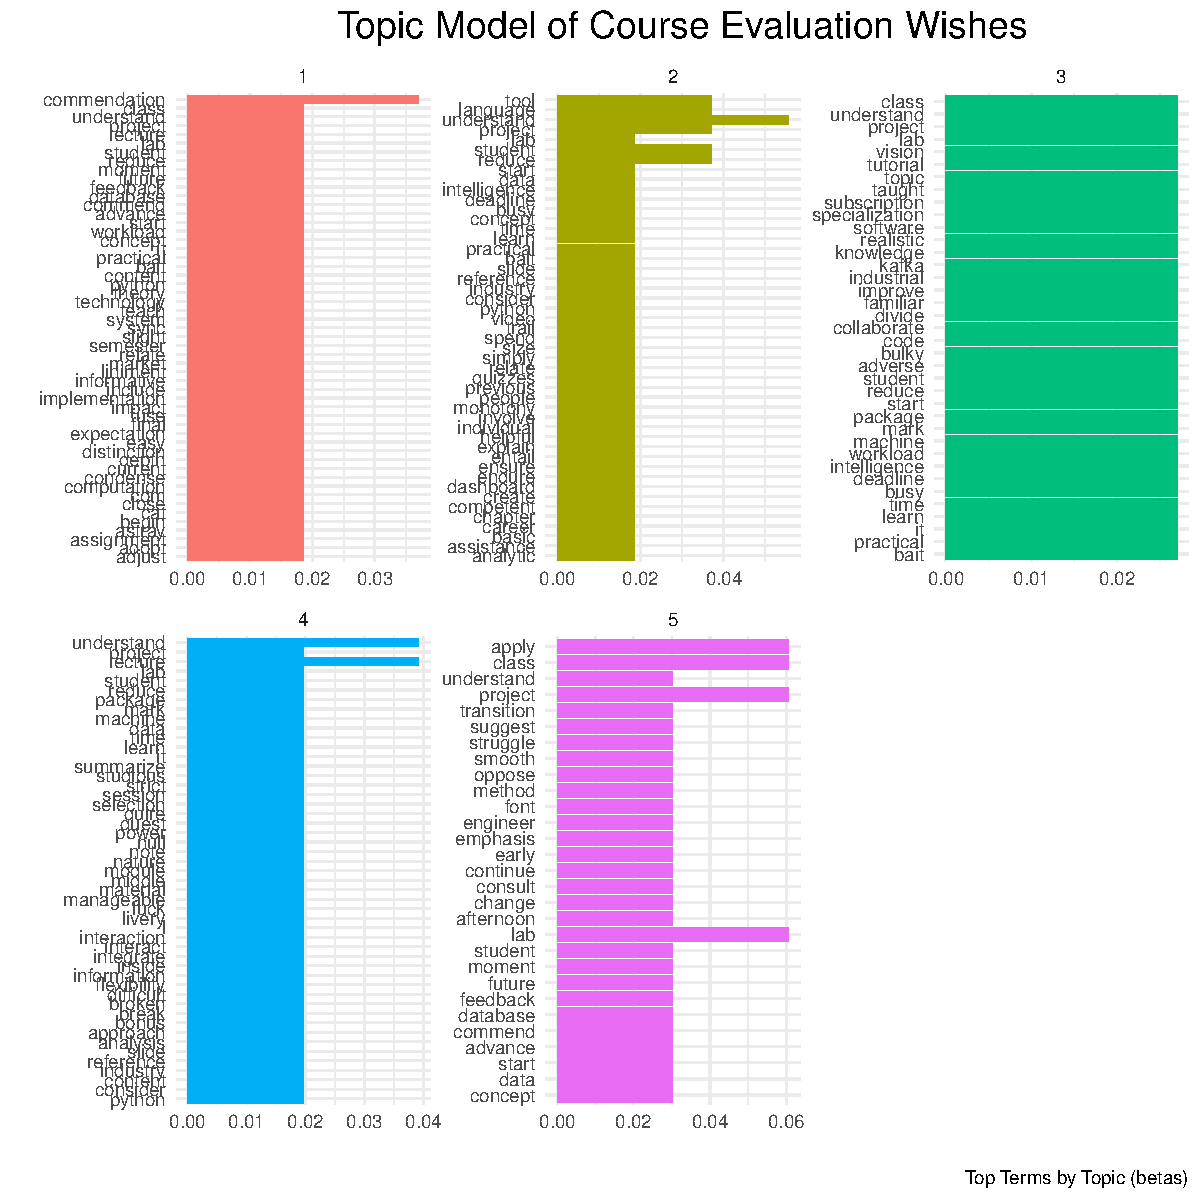
\includegraphics{10.b.BBT4206-End-SemesterCourseEvaluation-20230821-20231128-BI2-BBIT4-2_files/figure-latex/visualizations_for_wishes_topic_modelling-1.pdf}

\newpage

The 3 topics for the recommended BI content (as guided by the LDA model)
are:

\begin{enumerate}
\def\labelenumi{\arabic{enumi}.}
\item
  Topic 1: Python
\item
  Topic 2: Tableau
\item
  Topic 3: PowerBI
\end{enumerate}

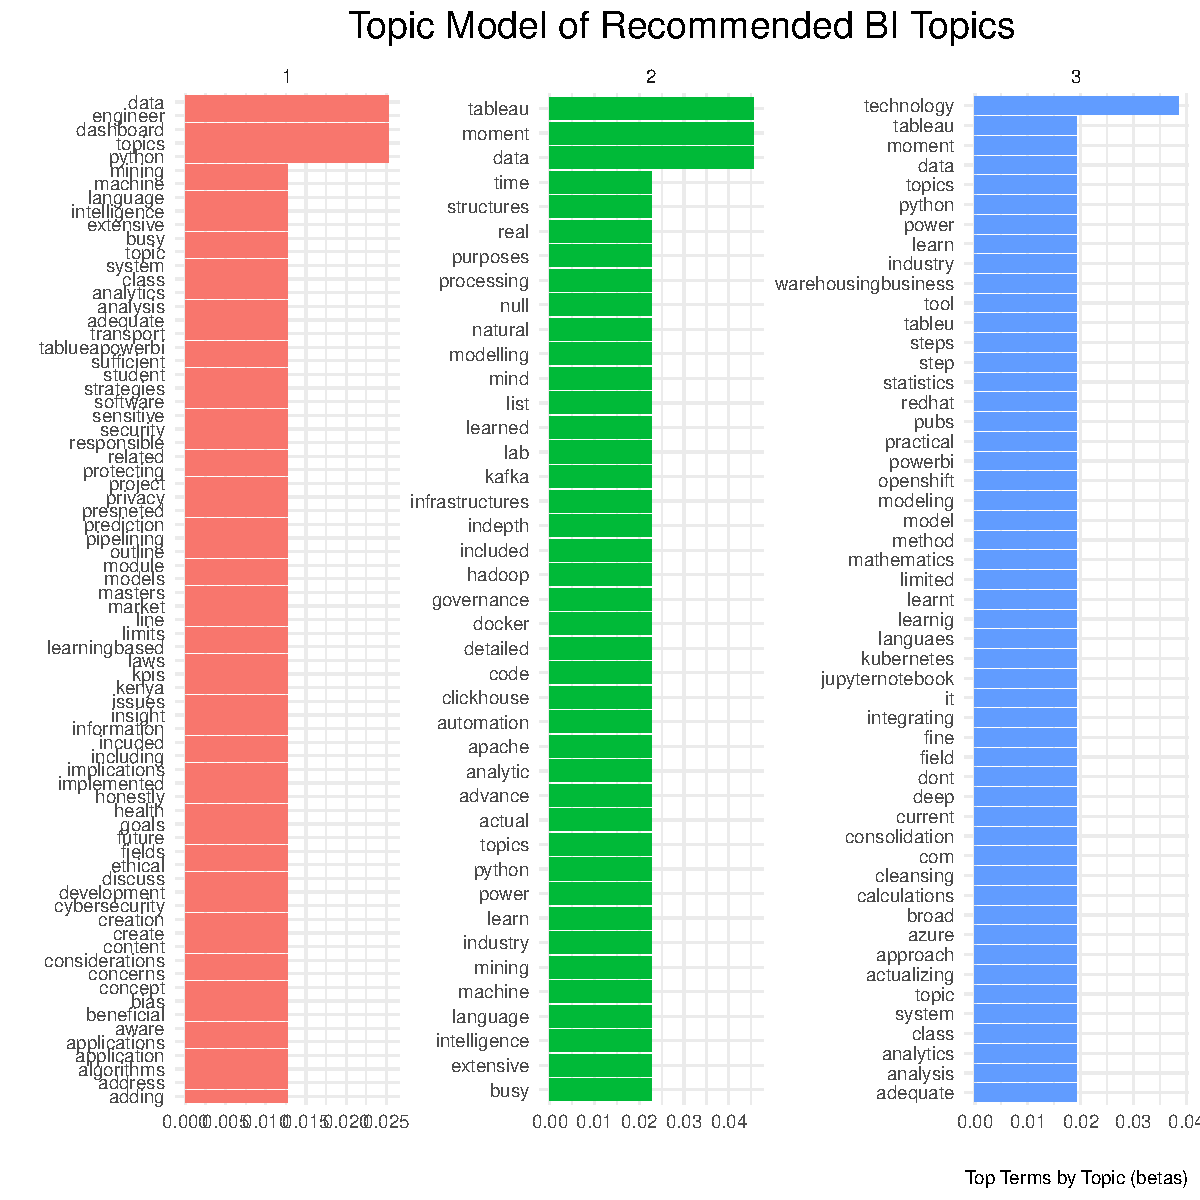
\includegraphics{10.b.BBT4206-End-SemesterCourseEvaluation-20230821-20231128-BI2-BBIT4-2_files/figure-latex/visualizations_for_recommended_topics_topic_modelling-1.pdf}

\newpage

\section{Appendices}\label{appendices}

\subsection{Appendix A: Full Name of
Variables}\label{appendix-a-full-name-of-variables}

The following variables have been renamed to fit the correlation plots:

\begin{itemize}
\item
  `A. Enjoying Subject` = `Q02\_General Questions-\textgreater A - 1. I
  enjoyed the subject`,
\item
  `B. Classes Start-End` = `Q02\_General Questions-\textgreater A - 2.
  Classes started and ended on time`,
\item
  `C. Learning Environment` = `Q02\_General Questions-\textgreater A -
  3. The learning environment was participative, involved learning by
  doing and was group-based`,
\item
  `D. Content Delivery` = `Q02\_General Questions-\textgreater A - 4.
  The subject content was delivered according to the course outline and
  met my expectations`,
\item
  `E. Clear Topics` = `Q02\_General Questions-\textgreater A - 5. The
  topics were clear and logically developed`,
\item
  `F. Oral and Writing` = `Q02\_General Questions-\textgreater A - 6. I
  developed my oral and writing skills`,
\item
  `G. Critical Thinking` = `Q02\_General Questions-\textgreater A - 7. I
  developed my reflective and critical reasoning skills`,
\item
  `H. Assessment Methods` = `Q02\_General Questions-\textgreater A - 8.
  The assessment methods assisted me to learn`,
\item
  `I. Relevant Feedback` = `Q02\_General Questions-\textgreater A - 9. I
  received relevant feedback`,
\item
  `J. Read Recommendations` = `Q02\_General Questions-\textgreater A -
  10. I read the recommended readings and notes`,
\item
  `L. eLearning Material` = `Q02\_General Questions-\textgreater A - 11.
  I used the eLearning material posted`,
\item
  `Understood BI1 Concept 1` = `Q03\_Level of Learning
  Achieved-\textgreater B - 1. - BI1 - Concept 1 of 4: Ensemble Methods
  for Predictive Analytics`,
\item
  `Understood BI1 Concept 2` = `Q03\_Level of Learning
  Achieved-\textgreater B - 2. - BI1 - Concept 2 of 4: Linear Algorithms
  for Predictive Analytics`,
\item
  `Understood BI1 Concept 3` = `Q03\_Level of Learning
  Achieved-\textgreater B - 3. - BI1 - Concept 3 of 4: Non-Linear
  Algorithms for Predictive Analytics`,
\item
  `Understood BI1 Concept 4` = `Q03\_Level of Learning
  Achieved-\textgreater B - 4. - BI1 - Concept 4 of 4: Dashboarding for
  Business-Facing and Customer-Facing Analytics`,
\item
  `Understood BI2 Concept 1` = `Q03\_Level of Learning
  Achieved-\textgreater B - 1. - BI2 - Concept 1 of 4: Ensemble Methods
  for Predictive Analytics`,
\item
  `Understood BI2 Concept 2` = `Q03\_Level of Learning
  Achieved-\textgreater B - 2. - BI2 - Concept 2 of 4: Predictive
  Modelling Using R`,
\item
  `Understood BI2 Concept 3` = `Q03\_Level of Learning
  Achieved-\textgreater B - 3. - BI2 - Concept 3 of 4: Data Warehousing
  and BI Strategy Implementation`,
\item
  `Understood BI2 Concept 4` = `Q03\_Level of Learning
  Achieved-\textgreater B - 4. - BI2 - Concept 4 of 4: Data
  Engineering`,
\item
  `Acquired Skill 1` = `Q04\_Competency for Technologies-\textgreater D
  - 1. ChartJS`,
\item
  `Acquired Skill 2` = `Q04\_Competency for Technologies-\textgreater D
  - 2. R (includes R markdown and R plumber)`,
\item
  `Acquired Skill 3` = `Q04\_Competency for Technologies-\textgreater D
  - 3. MySQL`,
\item
  `Acquired Skill 4` = `Q04\_Competency for Technologies-\textgreater D
  - 4. Kafka`,
\item
  `Acquired Skill 5` = `Q04\_Competency for Technologies-\textgreater D
  - 5. ksqlDB`,
\item
  `Acquired Skill 6` = `Q04\_Competency for Technologies-\textgreater D
  - 6. ClickHouse`,
\item
  `Acquired Skill 7` = `Q04\_Competency for Technologies-\textgreater D
  - 7. Linear and Non-Linear ML Algorithms in the caret package`,
\item
  `Group Project` = `Q05\_Quality of Teaching Strategies-\textgreater E
  - 1. Group project`,
\item
  `Labs Manuals` = `Q05\_Quality of Teaching Strategies-\textgreater E -
  2. Lab manuals that outline the steps to follow during the labs`,
\item
  `Lab Submissions` = `Q05\_Quality of Teaching
  Strategies-\textgreater E - 3. Required lab work submissions at the
  end of each lab manual that outline the activity to be done on your
  own`,
\item
  `Supplementary Videos/Audio` = `Q05\_Quality of Teaching
  Strategies-\textgreater E - 4. Supplementary videos/audio to
  watch/listen to`,
\item
  `Lecture Slides` = `Q05\_Quality of Teaching Strategies-\textgreater E
  - 5. Lectures slides`,
\item
  `Lecture Notes` = `Q05\_Quality of Teaching Strategies-\textgreater E
  - 6. Lecture notes on some of the lecture slides`,
\item
  `Quality of Lectures` = `Q05\_Quality of Teaching
  Strategies-\textgreater E - 7. The quality of the lectures given
  (quality measured by the breadth (the full span of knowledge of a
  subject) and depth (the extent to which specific topics are focused
  upon, amplified, and explored) of learning - NOT quality measured by
  how fun/comical the lectures are)`,
\item
  `Online for Theory` = `Q05\_Quality of Teaching
  Strategies-\textgreater E - 8. The division of theory and practice
  such that most of the theory is done during the recorded online
  classes and most of the practice is done during the physical classes`,
\item
  `Recording of Online` = `Q05\_Quality of Teaching
  Strategies-\textgreater E - 9. The recordings of online classes`
\end{itemize}

\newpage

\subsection{Appendix B: Raw Qualitative
Data}\label{appendix-b-raw-qualitative-data}

\subsubsection{Likes}\label{likes}

The raw data of the likes is as follows:

\ldots gin\{longtable\}{[}t{]}\{\textgreater\{

\raggedright

\arraybackslash\}p\{35em\}\}

\caption{\label{tab:RawLikesData}Write two things you like about the teaching and learning in this unit so far}

\textbackslash{} \toprule Comment (Likes)\textbackslash{} \midrule
Improved my knowledge on R markdown As well as Knowledge Discovery in
Databases\textbackslash{} \hline It was interactive and engaging~ the
leacturer gave clear and easy to understand materials\textbackslash{}
\hline Organized, Extensive\textbackslash{} \hline Group lab workThe
lecturer's detail\textbackslash{} \hline \emph{- It was practical and
engaging - use of github for collaboration\textbackslash{} \hline The
teaching stye The labs\textbackslash{} \hline - It was very practical~ -
The concepts were few hence easier internalization and
practice\textbackslash{} \hline it was board and well understood,
atleast by me it can be used for my future career as a data
analyst\textbackslash{} \hline }-Classes began and ended on time -
Lecturer was free with questions\textbackslash{} \hline It was so
engaging and informative\textbackslash{} \hline Lecturer was
Insightful\textbackslash{} \hline time management\textbackslash{} \hline
The level of teaching by the lecturer~\textbackslash{} \hline
1. Comprehensive 2. Detailed\textbackslash{} \hline How extensive it was
Good delivery\textbackslash{} \hline The power point was easy to
understand.\textbackslash{} \hline Comprehensive Introduction and use of
GitHub and Collaborations tools as a Version Control System.~ Learning R
and R studio and also road towards being a Data
Engineer.~\textbackslash{} \hline The organized delivery of content.
~\textbackslash{} \hline The applicability~The knowledge gained about
the industry\textbackslash{} \hline The labs~ That the practical side
was taught in class\textbackslash{} \hline The lecture cares which is
not most common in University. Keep caring sir it helps students learn
better.\textbackslash{} \hline It was more on the practical side so it
was interesting to learn in that way Ample time was given to finish the
project\textbackslash{} \hline Lab activities Tasks given boosted
learning\textbackslash{} \hline I liked that the teaching and learning
was very involving in the class and was group-based. I liked that it
helped me in choosing my career path.\textbackslash{} \hline Learning
about different models~ The teaching assessments was done in form of
groups\textbackslash{} \hline I appreciated the personalized learning
approach the lecturer offered each student in case of challenges. I
appreciated the flexibility of the deadlines of the labs and projects.
~\textbackslash{} \hline The unit was very practical The labs were
organized in an excellent manner that assisted in clear understanding of
the R language\textbackslash{} \hline Hands on labs use of current
technologies\textbackslash{} \hline Group labs created a platform to
gain different perspectives from other students lab tutorials were
detailed allowing for easy understanding of the content\textbackslash{}
\hline The lecturer always provided help where possible.~ The lecturer
was organized making it easier to understand the unit. The lecturer was
dedicated and loved teaching.\textbackslash{} \hline \emph{- the unit
was taught very comprehensively. - the unit was very educative in
relation to real world application such as dashboarding and Data
analytics.\textbackslash{} \hline The in depth of the content and the
practical labs~\textbackslash{} \hline The content The Teaching
style\textbackslash{} \hline The lecturer found a way to have recordings
available to us despite the challenges on storage, and set aside
consultation hours for one to~ go conslult.~He made the learning
environment~ safe sapce to make mistkes and say wrng answer and give
one's thoughts\textbackslash{} \hline Classes were engaging Detailed lab
instructions\textbackslash{} \hline good~ explanation\textbackslash{}
\hline involvment with the students\textbackslash{} \hline mode of
delivery practicals but not that much\textbackslash{} \hline The mode of
delivery The way the topics were logically developed\textbackslash{}
\hline The student - teacher relation in regards to academics The
avaliabillity of multiple content\textbackslash{} \hline Group
work\textbackslash{} \hline The notes were provided before the classes
The lecturer took time to teach which helped in understanding the
concepts\textbackslash{} \hline The lecturer is well endowed with the
concepts and this made it easy to understand. The labs allowed me to
think outside the box and this was nice.\textbackslash{} \hline The
detailed information given when learning the labs~ The participative
environment\textbackslash{} \hline doing the labs quizzes after each
topic\textbackslash{} \hline The labs were informative The lectures were
thorough~\textbackslash{} \hline The interactiveness\textbackslash{}
\hline The lecturer explains the concepts well The classes are very
interesting\textbackslash{} \hline The unit did have a lot of content
but the content was also very educative and enabled me to know about BI.
The lecturer taught the unit well and all the information put across
well.\textbackslash{} \hline Very Organised\textbackslash{} \hline
\ldots\textbackslash{} \hline Labs and projects Material shared helped
me learn\textbackslash{} \hline Intelligence\textbackslash{} \hline
Class engagement\textbackslash{} \hline Well explained topics. GitHub
relation to the labs done.\textbackslash{} \hline clear showing of the
practical conceptsclearly showed hoe to use GitHub for
teams\textbackslash{} \hline
1. The group work 2. The labs and even the explanation and teaching of
the labs was well done\textbackslash{} \hline The depth of knowledge and
content shared is really impressive.\textbackslash{} \hline
N/A\textbackslash{} \hline The KDD process and the practical
learning\textbackslash{} \hline Practise materials and
lessons\textbackslash{} \hline Learning R langauge and how we can play
with data~\textbackslash{} \hline I learnt Rand how data analytics is
all about\textbackslash{} \hline Group assignment via the
github~\textbackslash{} \hline the interactive lab works and the
quizes\textbackslash{} \hline The learning environment was participative
The lecturer explained the concepts well ~\textbackslash{} \hline Every
concept taught was explained extensive and tested~ The Lab work were
really good which I was able to gather knowledge and skills that I can
use in my future or even to expand the knowledge in that field
~\textbackslash{} \hline technical hands on labs improved knowledge on
data analysis\textbackslash{} \hline The practical labs on GitHub made
me competent on how to use such tools. Learning how to use R something
that can be added on my CV.\textbackslash{} \hline The practical side of
learning using the labs The projects help me learn a lot\textbackslash{}
\hline the labs were developed very thoughtfully to build technical and
collaborative skills~ the concepts were thoroughly explained especially
in the labs with relavant real world applications~\textbackslash{}
\hline Thorough content Practicality~\textbackslash{} \hline the lab
work submission instructions on the document coordination in
github\textbackslash{} \hline understanding and helpful\textbackslash{}
\hline The unit was delivered well. The practical side of the unit was
well explained\textbackslash{} \hline The lecturer is keen to make sure
no student is left behind. The learning is very practical thus allowing
students to learn for themselves.\textbackslash{} \hline lecture slides
group projects\textbackslash{} \hline Interactive\textbackslash{} \hline
the lecturers panctuality. the mode of teaching\textbackslash{} \hline
Composure of lecturer, His need for us to learn processes that are
applicable to the job market, e.g.~Github\textbackslash{} \hline I liked
that the lecturer was so clear and precise in the content he gave us, it
was adequate and you could tell that it made sense~ I liked that he went
out of his way to teach us extra concepts that will help us in our
carreer, that was very thoughtful of him.\textbackslash{} \hline Topics
were well explained\textbackslash{} \hline
1. The lectures started and ended in time, leaving room to ask the
lecturer for further assistance if one is stuck. 2. The Lecturer
responded to emails in a very convenient and timely
manner.\textbackslash{} \hline Model DesignR-programing\textbackslash{}
\hline Lab work and lectures\textbackslash{} \hline Lab
Exercises\textbackslash{} \hline I liked doing the labs and
quizzes\textbackslash{} \hline The practicals offered in class during
the lessonsN/A~\textbackslash{} \hline }-the practicals -the detailed
notes\textbackslash{} \hline I liked the learning in general, very
interesting topics were discussed\textbackslash{} \hline I liked how
each of the topics and labs were broken down\textbackslash{} \hline Good
lecturer~\textbackslash{} \hline The group work interaction. Learning
new skills. The lecturer is so skilled.Bravo!\textbackslash{} \hline -I
liked the fact that we learned R~\textbackslash{} \hline very organised.
reflects how the industry works especially BI 2\textbackslash{} \hline
The depth of the labs from start to end The unit project that helped to
apply all the knowledge\textbackslash{} \hline The topics were
extensively taught\textbackslash{} \hline The method used to deliver
content was highly inclusive\textbackslash{} \hline How the labs guided
us to learning R The labs also taught us to use Github\textbackslash{}
\hline Very organized and ready to help~\textbackslash{} \hline The
group projects made me understand the content better.\textbackslash{}
\hline very comprehensive~\textbackslash{} \hline the group-based
activities\textbackslash{} \hline Very practical subject that can be
used in the future The organization of the lecturers teaching
materials\textbackslash{} \hline The lecturer attended to all our
queries and questions The lecturer gave us additional materials for
revision\textbackslash{} \hline
1. relevant feedback 2. content was well and logically
explained\textbackslash{} \hline The practical nature. The teaching
method and effort relayed by the lecturer, Dr.~Allan
Omondi.\textbackslash{} \bottomrule \textbackslash end\{longtable\}

\newpage

\subsubsection{Wishes}\label{wishes}

The raw data of the wishes is as follows:

\ldots gin\{longtable\}{[}t{]}\{\textgreater\{

\raggedright

\arraybackslash\}p\{35em\}\}
\textbackslash caption\{\label{tab:RawWishesData}Write at least one
recommendation to improve the teaching and learning in this unit (for
the remaining weeks in the semester).\textbackslash{} \toprule Comment
(Wishes)\textbackslash{} \midrule None.\\
\hline Alittle more tutorials before starting a different topic or
project would help adversly to get familiar with it\textbackslash{}
\hline Flexibility,\textbackslash{} \hline The group project has to be
better integrated with the BI project so as to mean that BI doesn't have
to be srtictly seen through one lense as was the case in this
lecture\textbackslash{} \hline use of various data analytics
tools\textbackslash{} \hline Classes are ok as they are~\textbackslash{}
\hline \emph{- Sync the project and labs for easier implementation of
concepts as was done in advanced database systems\textbackslash{} \hline
i dont have any\textbackslash{} \hline }-None\textbackslash{} \hline
Provision of student packages to software that run on
subscription.\textbackslash{} \hline Maybe the lecturer can be more
intreractive\textbackslash{} \hline collaborative learning in
class~\textbackslash{} \hline N/A\textbackslash{} \hline Longer
deadlines.\textbackslash{} \hline Reduce the workload just abit, and
improve how course work marks are divided\textbackslash{} \hline Please
please, make the labs understandable there was too much information I
could not understand anything.\textbackslash{} \hline At the moment
everything is okay~\textbackslash{} \hline N/A\textbackslash{} \hline A
bit more assistance in regards to the BI project\textbackslash{} \hline
Less group work\textbackslash{} \hline I would suggest doing the project
throughout the course like it was done in Advanced Database where each
lab applies to a students project so on and so forth which may help
students understand better as they apply it to their
projects.~\textbackslash{} \hline Feedback\textbackslash{} \hline More
lab sessions Interaction with the industry\textbackslash{} \hline I
would recommend for the same methods used to continue for future
classes.\textbackslash{} \hline Be able to consult students and know
what they are struggling with in order to help them understand the
course a lot more\textbackslash{} \hline N/A\textbackslash{} \hline I
would recommend the unit to be done in a `LAB'\textbackslash{} \hline
n/a\textbackslash{} \hline For a distinction between labs and theory in
order to well understand the computations~\textbackslash{} \hline The BI
unit to be~ taught early from maybe third year since it is a
specialization unit. This will help with understanding the unit better
since it is bulky and getting more industrial knowledge like
understanding kafka and more. The BI project especially the coding, to
start early so that we get more time to do the project
well.\textbackslash{} \hline \emph{- more reference
materials.\textbackslash{} \hline For labs, earlier classes in the day
as opposed to afternoon classes~\textbackslash{} \hline
None\textbackslash{} \hline No comment\textbackslash{} \hline
N/A\textbackslash{} \hline n/a\textbackslash{} \hline
none\textbackslash{} \hline Content is too much. Reduce the content and
nature of the labs\textbackslash{} \hline Good Luck\textbackslash{}
\hline Make up Cats\textbackslash{} \hline None\textbackslash{} \hline
No more recommendations\textbackslash{} \hline Nothing should
change.\textbackslash{} \hline More empasis on the data engineering
concept\textbackslash{} \hline add bonus marks\textbackslash{} \hline
The labs should keep on being done in groups\textbackslash{} \hline The
software we use are unrealistic~ in way they can't run on my machine,if
there were provision of machine or the labs it would be
good\textbackslash{} \hline Business Intelligence to be more
practical\textbackslash{} \hline Maybe learning more about coding in
R\textbackslash{} \hline it is good as is\textbackslash{} \hline
\ldots\textbackslash{} \hline Since we only start working with R in BI
2. Students can start learning R during BI 1. This will help them have a
good understanding of the basics of R, such that in BI 2 they will
understand better the labs and be able to do the labs and projects well.
They'll also be competent in R, which will be helpful in their careers
industry\textbackslash{} \hline .\textbackslash{} \hline Student
involvement\textbackslash{} \hline More group work\textbackslash{}
\hline I have no recommendations\textbackslash{} \hline
1. Selections to be early~\textbackslash{} \hline Concept 2 of
4(BI2)went astray from my expectations of the unit. It was very
informative but it was too long and there was a lot of content to work
through. Probably for future groups, it can be done away with or the
content condensed. Also using Python would be better than using
R.\textbackslash{} \hline N/A\textbackslash{} \hline Reduce the
workload. Final year students have so much work and the BI lecturer
didn't seem to adjust his relative to his students\textbackslash{}
\hline More feedback on the assignments given\textbackslash{} \hline
N/A\textbackslash{} \hline A video that will simply entail all that will
be done in Business Intelligence - like a trailer.\textbackslash{}
\hline The notes inside the labs(RStudio) to be summarized in
powerpoint\textbackslash{} \hline N/A\textbackslash{} \hline the slides
to be well explained\textbackslash{} \hline Nothing at the
moment\textbackslash{} \hline N/A\textbackslash{} \hline The time used
in explaining the first previous chapters can be reduced to endure that
student does not get that monotony of what has already been done. Use of
other languages as Python but R can be used as the reference tool and
language.\textbackslash{} \hline Machine learning with python and
learning python data analysis packages\textbackslash{} \hline that the
project be different from the IS project, doing both project
concurrently is confusing\textbackslash{} \hline None\textbackslash{}
\hline None at the moment\textbackslash{} \hline n/a\textbackslash{}
\hline For practicals adopt using new technologies that are being used
in the job market.\textbackslash{} \hline The project and labs are too
many and require a lot of work in very little time which is difficult
with what students already have going on with other units I request the
lecturer considers making them more manageable.\textbackslash{} \hline
Reduce the size of the project because some people might not be doing an
IS project relating to BI\textbackslash{} \hline I think it is
ok\textbackslash{} \hline put a break in the middle of the lecture not
towards the end of it\textbackslash{} \hline Have all the labs be
individual, ensures that everyone actually understands the
concepts.~\textbackslash{} \hline The class was impactful by teaching us
using R however a ix of R and python would have really gone a long
way.\textbackslash{} \hline The labs were good maybe reduce them a abit
How to create the dashboards practically Quizes to be done at the end of
each concept like BI 1\textbackslash{} \hline
1. Deadlines for the labs should be considered.\textbackslash{} \hline
Null\textbackslash{} \hline n/a\textbackslash{} \hline
None\textbackslash{} \hline The slides could be a broken down a bit more
so that not all the content is in one set\textbackslash{} \hline The
project to begin at the start of the semester not close to the
end\textbackslash{} \hline No reccomendation\textbackslash{} \hline
Reduce the workload\textbackslash{} \hline none\textbackslash{} \hline
None\textbackslash{} \hline None.\textbackslash{} \hline }Spend more
times on labs\textbackslash{} \hline if we can start some labs in BI 1
for a smooth transtion in BI2\textbackslash{} \hline Github group labs
were abit confusing to work with\textbackslash{} \hline
N/A\textbackslash{} \hline Different approaches towards delivery of som
of the modules\textbackslash{} \hline N/A\textbackslash{} \hline
Everything is in order\textbackslash{} \hline .\textbackslash{} \hline
Using Python~\textbackslash{} \hline there should not be a lot of work
lecturer should be abit linient\textbackslash{} \hline
N/A\textbackslash{} \hline To include Python\textbackslash{} \hline i
have none\textbackslash{} \hline Reduce the content depth
slightly.\textbackslash{} \bottomrule \textbackslash end\{longtable\}

\newpage

\subsection{Appendix C: Additional Topics to Include in the
Course}\label{appendix-c-additional-topics-to-include-in-the-course}

The raw data of the addtional topics to include is as follows:

\ldots gin\{longtable\}{[}t{]}\{\textgreater\{

\raggedright

\arraybackslash\}p\{35em\}\}

\caption{\label{tab:AdditionalTopics}Are there any topics that you recommend should be added to in addition to the ones already in the BI1 and BI2 course outlines?}

\textbackslash{} \toprule List of Topics\textbackslash{} \midrule
None.\\
\hline I would like to have learned about real time business
intelligence for real time data processing and maybe some advanced data
modelling\textbackslash{} \hline N/A\textbackslash{} \hline
None\textbackslash{} \hline use of python language use of
tabluea/powerbi\textbackslash{} \hline N/A\textbackslash{} \hline
None\textbackslash{} \hline none.that i know of\textbackslash{} \hline -
I honestly believe the content is sufficient even for a masters student
~\textbackslash{} \hline Natural Language processing\textbackslash{}
\hline N/A~\textbackslash{} \hline Real time analytic~\textbackslash{}
\hline Data Pipelining~\textbackslash{} \hline None that I can think of
at the moment\textbackslash{} \hline Real time BI\textbackslash{} \hline
Maybe Kafka in-depth\textbackslash{} \hline Nothing much to
add.~\textbackslash{} \hline Apache Hadoop Power BI\textbackslash{}
\hline Application to other fields apart from business e.g Health,
Transport etc\textbackslash{} \hline More python labs\textbackslash{}
\hline Cybersecurity in BI: Address the security concerns associated
with BI systems and data, including strategies for protecting sensitive
information. Ethical Considerations in BI: Discuss the ethical
implications of using BI, including issues related to privacy, bias, and
responsible data use.\textbackslash{} \hline Dashboards and kpis were in
the course outline but maybe they should have more insight on the limits
and goals a KPI should have.\textbackslash{} \hline R lab
works\textbackslash{} \hline The topics are okay as they
are.\textbackslash{} \hline Creation of prediction models in order to be
able to be implemented into different projects\textbackslash{} \hline
Tableau I think should be included I think for the purposes of
industry~\textbackslash{} \hline A topic on consolidation step that has
clear steps in integrating the model to the system and various methods
to approach it.\textbackslash{} \hline I believe the current topics are
fine\textbackslash{} \hline Data warehousing~business
modeling\textbackslash{} \hline none.\textbackslash{} \hline * Data
mining * Automation * Governance\textbackslash{} \hline
N/A\textbackslash{} \hline Use of python\textbackslash{} \hline No
Comment\textbackslash{} \hline NA\textbackslash{} \hline
n/a\textbackslash{} \hline as of right now i cant think of
any\textbackslash{} \hline none\textbackslash{} \hline Data
Ops\textbackslash{} \hline Practicals like actually going the the field
and actualizing what the has been learnt in class~\textbackslash{}
\hline I dont know\textbackslash{} \hline PowerBI\textbackslash{} \hline
The course outline is quite extensive and in line with the market. I
believe it will be beneficial for future classes as it
is.\textbackslash{} \hline The data engineering topic\textbackslash{}
\hline none\textbackslash{} \hline Can't think of any more it's quite
extensive~\textbackslash{} \hline Actual machine
learning~\textbackslash{} \hline Tableau\textbackslash{} \hline Coding
in R\textbackslash{} \hline How to use tableu R pubs\textbackslash{}
\hline \ldots\textbackslash{} \hline None. The topics presneted were
adequate\textbackslash{} \hline Algorithms\textbackslash{} \hline app
development\textbackslash{} \hline Machine
learning-based~\textbackslash{} \hline Use azure as it is a key
technology in the industry.\textbackslash{} \hline None in mind at the
moment~\textbackslash{} \hline Data Analysis using
Python\textbackslash{} \hline detailed structures on
infrastructures\textbackslash{} \hline Can't think of
any\textbackslash{} \hline Kubernetes , Redhat OpenShift
technologies\textbackslash{} \hline N/A\textbackslash{} \hline Kenya
Data laws\textbackslash{} \hline N/A\textbackslash{} \hline none that i
can think of\textbackslash{} \hline data analytics\textbackslash{}
\hline The concepts were extensive maybe just adding some Python lab
modules.\textbackslash{} \hline Business Intelligence with AI or
ML\textbackslash{} \hline Not aware of any topics that may be
incuded\textbackslash{} \hline None\textbackslash{} \hline using
industry tools such as power bi and tableau for data analytics~ using
newer languaes and technologies such as python for data
analytics~\textbackslash{} \hline None\textbackslash{} \hline Maybe try
using R\textbackslash{} \hline well all have been done\textbackslash{}
\hline Data Cleansing\textbackslash{} \hline I have no topics to add to
the list.\textbackslash{} \hline Applications of business intelligence
in software engineering\textbackslash{} \hline None\textbackslash{}
\hline the topics there are enough\textbackslash{} \hline
none~\textbackslash{} \hline Deep learnig~\textbackslash{} \hline How to
create good dashboards\textbackslash{} \hline
1. Business Intelligence I - None 2. Business Intelligence II -
None\textbackslash{} \hline Null\textbackslash{} \hline
N/A\textbackslash{} \hline The topics were enough\textbackslash{} \hline
How to use Docker and Clickhouse\textbackslash{} \hline
N/A\textbackslash{} \hline The topics are adequate\textbackslash{}
\hline None - the unit is rather broad as it is\textbackslash{} \hline
none\textbackslash{} \hline None\textbackslash{} \hline
None.\textbackslash{} \hline N/a\textbackslash{} \hline Data Mining and
Big Data Analysis\textbackslash{} \hline The course should not be
limited to R, should also allow Python where JupyterNotebook can be
learnt well\textbackslash{} \hline N/A\textbackslash{} \hline
N/A\textbackslash{} \hline ~N/A\textbackslash{} \hline They are all
okay\textbackslash{} \hline .\textbackslash{} \hline
NONE\textbackslash{} \hline none\textbackslash{} \hline
N/A\textbackslash{} \hline Deep learning\textbackslash{} \hline at the
moment none\textbackslash{} \hline Statistics, calculations,
mathematics\textbackslash{} \bottomrule \textbackslash end\{longtable\}

\end{document}
